\documentclass[
	% -- opções da classe memoir --
	12pt,				% tamanho da fonte
	a4paper,			% tamanho do papel.
	oneside,
	% -- opções do pacote babel --
	english			% idioma adicional para hifenização, o último idioma é o principal do documento
	]{abntex2}

% ---
% Pacotes básicos
% ---
\usepackage{lmodern}			% Usa a fonte Latin Modern
\usepackage[T1]{fontenc}		% Selecao de codigos de fonte.
\usepackage[utf8]{inputenc}		% Codificacao do documento (conversão automática dos acentos)
\usepackage{indentfirst}		% Indenta o primeiro parágrafo de cada seção.
\usepackage{color}				% Controle das cores
\usepackage{graphicx}			% Inclusão de gráficos
\usepackage{microtype} 			% para melhorias de justificação
% ---

\usepackage{url}

% ---
% Pacotes de citações
% ---
\usepackage[brazilian,hyperpageref]{backref}	 % Paginas com as citações na bibl
\usepackage[alf]{abntex2cite}	% Citações padrão ABNT

\usepackage[color]{coqdoc}
\usepackage{cspsymb}
\usepackage{amsmath}

% Proof trees in the style of the sequent calculus
\usepackage{bussproofs}

% Unnumbered theorem-like environments
\usepackage{amsthm}

\theoremstyle{definition}
\newtheorem*{definition}{Definition}

%%%%% Coq Proof Script Visualiser %%%%%

\usepackage{tabularx}
\usepackage[mathletters]{ucs}
%\usepackage[utf8x]{inputenc}
%\usepackage{unicode}
%\usepackage{fullpage}
\usepackage{multirow}
\usepackage{longtable, array}

\usepackage{textcomp} % required to use \textquotesingle

% The width of the coq step column
\providecommand{\stepcolwidth}{0.2}
% The width of the frac rule in coq style output
\providecommand{\rulewidth}{1.0}
% The frac rule thickness in coq style output
\providecommand{\rulethickness}{0.2}
% The margin strech for the table cells
\renewcommand{\arraystretch}{1.3}
% The horizontal alignment of proof situations
\providecommand{\coqpsvpsitalign}{\centering}
% The command for printing the frac rule in coq style output
\providecommand{\fracrule}{\rule{\rulewidth\hsize}{\rulethickness mm}}
% The command for generating a proof situation environment
\providecommand{\coqpsvpsit}[1]{\begin{minipage}[t]{0.7\textwidth}\coqpsvpsitalign#1\end{minipage}}

% Now we define the table headers
\providecommand{\coqpsvstephdr}{Next step in Coq}
\providecommand{\coqpsvsithdr}{\multicolumn{1}{>{\centering\arraybackslash}c|}{Proof situation}}

\newcolumntype{S}{m{\stepcolwidth\textwidth}}
\newcolumntype{P}{>{\coqpsvpsitalign\arraybackslash}p{0.700000\textwidth}}

%%%%%%%%%%%%%%%%%%%%%%%%%%%%%%%%%%%%%%%

% ---
% CONFIGURAÇÕES DE PACOTES
% ---

% ---
% Configurações do pacote backref
% Usado sem a opção hyperpageref de backref
\renewcommand{\backrefpagesname}{Citado na(s) página(s):~}
% Texto padrão antes do número das páginas
\renewcommand{\backref}{}
% Define os textos da citação
\renewcommand*{\backrefalt}[4]{
	\ifcase #1 %
		Nenhuma citação no texto.%
	\or
		Citado na página #2.%
	\else
		Citado #1 vezes nas páginas #2.%
	\fi}%
% ---

% ---
% Informações de dados para CAPA e FOLHA DE ROSTO
% ---
\titulo{A Theory for Communicating\\ Sequential Processes in Coq}
\autor{Carlos Alberto da Silva Carvalho de Freitas}
\local{Recife}
\data{2020}
\orientador{Gustavo Henrique Porto de Carvalho}
\instituicao{%
  Universidade Federal de Pernambuco
  \par
  Centro de Informática
  \par
  Bachelor in Computer Engineering}
\tipotrabalho{Monografia (Bacharelado)}
% O preambulo deve conter o tipo do trabalho, o objetivo,
% o nome da instituição e a área de concentração
\preambulo{
	A B.Sc. Dissertation presented to the Centro de Informática of
	Universidade Federal de Pernambuco in partial fulfillment of the requirements
	for the degree of Bachelor in Computer Engineering.
}
% ---


% ---
% Configurações de aparência do PDF final

% alterando o aspecto da cor azul
\definecolor{blue}{RGB}{41,5,195}

% informações do PDF
\makeatletter
\hypersetup{
     	%pagebackref=true,
		pdftitle={\@title},
		pdfauthor={\@author},
    	pdfsubject={\imprimirpreambulo},
	    pdfcreator={LaTeX with abnTeX2},
		pdfkeywords={abnt}{latex}{abntex}{abntex2}{trabalho acadêmico},
		colorlinks=true,       		% false: boxed links; true: colored links
    	linkcolor=blue,          	% color of internal links
    	citecolor=blue,        		% color of links to bibliography
    	filecolor=magenta,      		% color of file links
		urlcolor=blue,
		bookmarksdepth=4
}
\makeatother
% ---

% ---
% Posiciona figuras e tabelas no topo da página quando adicionadas sozinhas
% em um página em branco. Ver https://github.com/abntex/abntex2/issues/170
\makeatletter
\setlength{\@fptop}{5pt} % Set distance from top of page to first float
\makeatother
% ---

% ---
% Espaçamentos entre linhas e parágrafos
% ---

% O tamanho do parágrafo é dado por:
\setlength{\parindent}{1.3cm}

% Controle do espaçamento entre um parágrafo e outro:
\setlength{\parskip}{0.2cm}  % tente também \onelineskip

% ---
% compila o indice
% ---
\makeindex
% ---

% Definindo o hífen com um novo caractere matemático para corrigir espaçamento e tamanho do símbolo no "env math".
\mathchardef\mhyphen="2D

% Defining symbol for the CSP_Coq language.
\newcommand{\CSPcoq}{CSP\textsubscript{\textit{Coq}}}

% ----
% Início do documento
% ----
\begin{document}

% Seleciona o idioma do documento (conforme pacotes do babel)
\selectlanguage{english}

% Retira espaço extra obsoleto entre as frases.
\frenchspacing

% ----------------------------------------------------------
% ELEMENTOS PRÉ-TEXTUAIS
% ----------------------------------------------------------

% ---
% Capa
% ---
\imprimircapa
% ---

% ---
% Folha de rosto
% ---
\imprimirfolhaderosto
% ---

% ---
% Agradecimentos
% ---
\begin{agradecimentos}
This work would not have been possible without the teaching and guidance of my supervisor, Professor Gustavo Carvalho, to whom I thank especially for understanding the adverse conditions in which this work has been developed; a pandemic without precedence in the contemporary history. I also extend my thanks to the other professors at the Centro de Informática of Universidade Federal de Pernambuco, who value quality education and encourage students to seek knowledge on a daily basis.

I cannot fully express my gratitude to my parents, Píndaro and Rozilda. All I am and everything I have achieved to this day I owe them. The humble yet challenging wish of my late father, when I was only a few years old, for me to grow into a good person and make contributions to the society, has always resonated deeply with me. My mother's relentless encouragement of my education and the pride she bears in her voice when talking about me, inspires me everyday to be the best version of myself.

Finally, I want to give special thanks to the people with whom I shared closely my emotions during the entire graduation course -- my classmates and my girlfriend, Nínive. The friendship and companionship of these people not only renewed my strength day after day, but made this journey enjoyable in a way that I could never have foreseen. Knowing that I could count on them has made a huge difference, and it was yet another good reason to get up every morning.
\end{agradecimentos}
% ---

% ---
% RESUMOS
% ---

% resumo em inglês
\setlength{\absparsep}{18pt} % ajusta o espaçamento dos parágrafos do resumo
\begin{resumo}
 Theories of concurrency such as Communicating Sequential Processes (CSP) allow system specifications to be expressed clearly and analysed with precision. CSP specifications are typically analysed with the aid of FDR, a refinement checker (model checker) for CSP. However, the state explosion problem, common to model checkers in general, is a real constraint when attempting to verify system properties for large systems. An alternative is to check these properties via proof development. Sometimes these proofs will need to be developed with the aid of the user. This work provides an initial formalisation of CSP in the Coq proof assistant, and evaluates how this theory compares to other theorem prover-based frameworks for the process algebra CSP. We develop an infrastructure for declaring syntactically and semantically correct CSP specifications in Coq, in addition to traces refinement analysis with the support of the QuickChick tool. Besides that, our infrastructure also has a native support for process representation through Labelled Transition Systems (LTSs).

 \textbf{Keywords}: CSP. Coq. Process algebra. Proof assistant. Traces refinement. QuickChick.
\end{resumo}

% resumo em português
\begin{resumo}[Resumo]
 \begin{otherlanguage*}{brazil}
   Teorias de concorrência, tais como \emph{Communicating Sequential Processes} (CSP), permitem que especificações de sistemas sejam descritas com clareza e analisadas com precisão. Especificações em CSP são normalmente analisadas em FDR, um verificador de refinamentos (verificador de modelos) para CSP. No entanto, o problema da explosão de estados, comum a verificadores de modelo em geral, é uma limitação real na tentativa de verificar propriedades de um sistema complexo. Uma alternativa é avaliar essas propriedades através do desenvolvimento de provas. Em algumas situações, estas provas precisam ser criadas a partir da intervenção do usuário. Este trabalho fornece uma primeira formalização de CSP no assistente de provas Coq, além de compará-la com outros \emph{frameworks} baseados em provadores de teoremas para a álgebra de processos CSP. Portanto, criou-se uma infraestrutura para declarar especificações sintatica e semanticamente corretas de CSP em Coq, além de permitir análise de refinamento no modelo de \emph{traces} a partir do uso da ferramenta QuickChick. Adicionalmente, esta infraestrutura possui suporte nativo para a representação de processos por meio de sistemas de transições rotuladas (LTSs).

   \textbf{Palavras-chave}: CSP. Coq. Álgebra de processos. Assistentes de provas. Refinamento no modelo de \emph{traces}. QuickChick.
 \end{otherlanguage*}
\end{resumo}

% ---
% inserir lista de ilustrações
% ---
\pdfbookmark[0]{\listfigurename}{lof}
\listoffigures*
\cleardoublepage
% ---

% ---
% inserir lista de tabelas
% ---
\pdfbookmark[0]{\listtablename}{lot}
\listoftables*
\cleardoublepage
% ---

% ---
% inserir lista de abreviaturas e siglas
% ---
\begin{siglas}
	\item[CSP] Communicating Sequential Processes
	\item[FDR] Failures-Divergence Refinement
	\item[LTS] Labelled Transition System
	\item[SOS] Structured Operational Semantics
	\item[UTP] Unified Theories of Programming
\end{siglas}
% ---

% ---
% inserir o sumario
% ---
\pdfbookmark[0]{\contentsname}{toc}
\tableofcontents*
\cleardoublepage
% ---


% ----------------------------------------------------------
% ELEMENTOS TEXTUAIS
% ----------------------------------------------------------
\textual

% ----------------------------------------------------------
% Chapter 1
% ----------------------------------------------------------
\chapter{Introduction}
% ----------------------------------------------------------

Concurrency is an attribute of any system that allows multiple components to perform operations at the same time. The understanding of this property is essential in modern programming because major areas, such as distributed and real-time systems, rely on this concept to work properly. As a result, the variety of applications enabled by the concurrency feature is broad: aircraft and industrial control systems, routing algorithms, peer-to-peer networks, client-server applications and parallel computation, to name a few.

Since concurrent systems may have parts that execute in parallel, the combination of ways in which these parts can interact raises the complexity in designing such systems. Phenomena like deadlock, livelock, nondeterminism and race condition can emerge from these interactions, so these issues must be addressed in order to avoid undesired behavior. Typically, testing cannot provide enough evidence to guarantee properties such as deadlock freedom, divergence freedom and determinism for a given system.

That being said, CSP (a theory for Communicating Sequential Processes) introduces a convenient notation that allows systems to be described in a clear and accurate way. More than that, it has an underlying theory that enables designs to be analysed and proven correct with respect to desired properties. The FDR (Failures-Divergence Refinement) tool is a model checker for CSP responsible for making this process algebra a practical tool for specification, analysis and verification of systems. System analysis is achieved by allowing the user to make assertions about processes and then exploring every possible behavior, if necessary, to check the truthfulness of the assertions made.

Although it is undeniable that FDR is a useful tool in the analysis of systems described in CSP, it has a limitation common to standard model checkers in general: the state explosion problem. An alternative way for deciding whether a system meets its specification is by proof development. Examples of this different approach are CSP-Prover and Isabelle/UTP, both frameworks based on the theorem prover Isabelle. Nevertheless, to the best of our knowledge, there is not a theory for CSP in the Coq proof assistant yet. Considering that, the main research question of this work is the following: how could we develop a theory of CSP in Coq, exploiting the main advantages of this proof assistant?

% ---
\section{Objectives}
% ---

The main objective (MO) of this work is to define in Coq a theory for concurrent systems, based on a limited scope of the process algebra CSP. This objective is unfolded into the following specific objectives (SO):

\begin{itemize}
	\item SO1: study CSP and frameworks based on this process algebra.
	\item SO2: define a syntax for CSP in Coq, based on a restricted version of the \CSPM{} language (machine readable language for CSP).
	\item SO3: provide support for the LTS-based (Labelled Transition System) representation, considering the Structured Operational Semantics (SOS) of CSP.
	\item SO4: make use of the QuickChick tool to search for counterexamples of the traces refinement relation.
\end{itemize}

% ---
\section{An overview of \CSPcoq{}}
% ---


Consider the following CSP process adapted from \citeonline[p.~32, example 2.3]{schneider1999}. This process represents a cloakroom attendant that might help a costumer off or on with his coat, storing an retrieving coats as appropriate:
\begin{align}
	\mathit{channel\ coat\_on, coat\_off, store, retrieve, request\_coat, eat}\notag
\end{align}
\begin{align}
	\mathit{SYSTEM} =\ &\mathit{coat\_off \mathbin{{-}{>}} store \mathbin{{-}{>}} request\_coat \mathbin{{-}{>}} retrieve \mathbin{{-}{>}} coat\_on \mathbin{{-}{>}} SKIP}\notag\\
			 &[|\ \{\mathit{coat\_off, request\_coat, coat\_on}\}\ |]\notag\\
	  		 &\mathit{coat\_off \mathbin{{-}{>}} eat \mathbin{{-}{>}} request\_coat \mathbin{{-}{>}} coat\_on \mathbin{{-}{>}} SKIP}\notag
\end{align}

We can declare such system in \CSPcoq{} by defining a specification, which consists in lists of channels and processes. This specification must also abide by a set of contextual rules that will be discussed further in this work.

\begin{coqdoccode}
	\coqdocnoindent
	\coqdockw{Definition} \coqdocvar{example} : \coqdocvar{specification}.\coqdoceol
	\coqdocnoindent
	\coqdockw{Proof}.\coqdoceol
	\coqdocindent{1.00em}
	\coqdocvar{solve\_spec\_ctx\_rules} (\coqdoceol
	\coqdocindent{2.00em}
	\coqdocvar{Build\_Spec}\coqdoceol
	\coqdocindent{2.00em}
	[ \coqdocvar{Channel} \{\{``coat\_off'', ``coat\_on'', ``request\_coat'', ``retrieve'', ``store'', ``eat''\}\} ]\coqdoceol
	\coqdocindent{2.00em}
	[ ``SYSTEM'' ::=\coqdoceol
	\coqdocindent{3.00em}
	``coat\_off'' --> ``store'' --> ``request\_coat'' --> ``retrieve'' --> ``coat\_on'' --> \coqdocvar{SKIP}\coqdoceol
	\coqdocindent{3.00em}
	[| \{\{``coat\_off'', ``request\_coat'', ``coat\_on''\}\} |]\coqdoceol
	\coqdocindent{3.00em}
	``coat\_off'' --> ``eat'' --> ``request\_coat'' --> ``coat\_on'' --> \coqdocvar{SKIP} ]\coqdoceol
	\coqdocindent{1.00em}
	).\coqdoceol
	\coqdocnoindent
	\coqdockw{Defined}.\coqdoceol
\end{coqdoccode}

Furthermore, we can execute the following command to compute the process LTS and output the graph in dot language:

\begin{coqdoccode}
	\coqdocnoindent
	\coqdockw{Compute} \coqdocvar{generate\_dot} (\coqdocvar{compute\_ltsR} \coqdocvar{example} ``SYSTEM'' 100).\coqdoceol
\end{coqdoccode}

The \autoref{lts-example} is a visual representation of the graph outputted by this command. The image is generated using GraphViz software.

\begin{figure}[htb]
	\caption[The process LTS graph]{The process LTS graph.}
	\label{lts-example}
	\begin{center}
		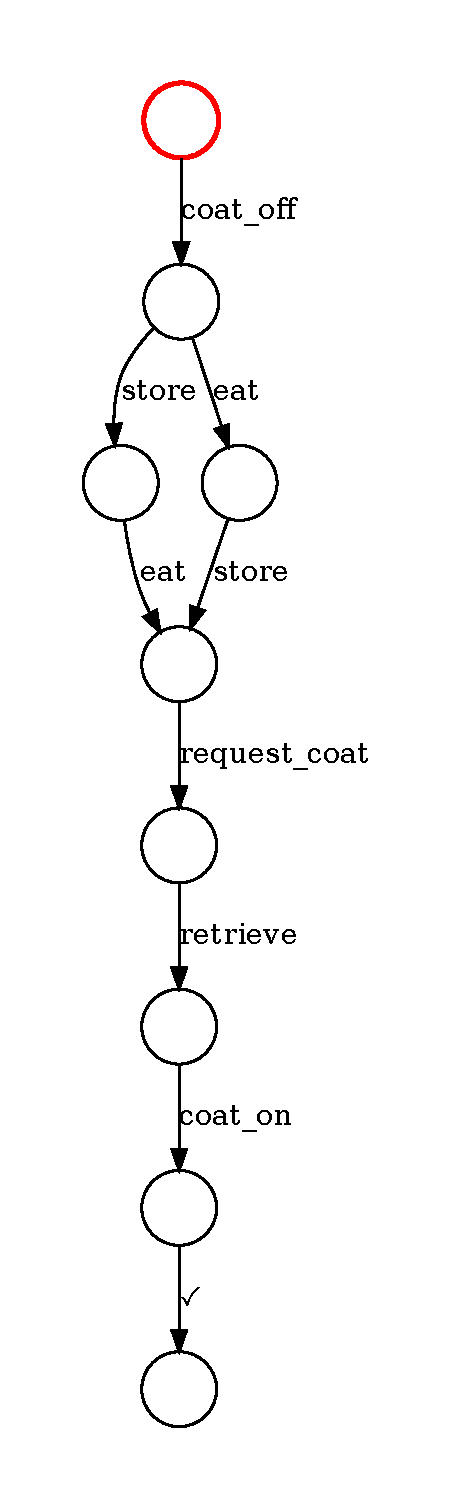
\includegraphics[scale=0.5]{images/LTS.pdf}
	\end{center}
\end{figure}

% ---
\section{Main contributions}
% ---

The main contributions of this work are the following:

\begin{itemize}
	\item Abstract and concrete syntax for a subset of CSP operators.
	\item Context rules for CSP specifications.
	\item Operational semantics via SOS approach.
	\item Inductive and functional definitions of a labelled transition system.
	\item Proof of correctness for the functional definition of the LTS.
	\item Inductive and functional definitions of traces.
	\item Proof of correctness for the functional definition of traces.
	\item Tactic macro that automates trace relation proofs.
	\item Formal definition of the traces refinement.
	\item Refinement verification using QuickChick.
\end{itemize}

% ---
\section{Document structure}
% ---

Apart from this introductory chapter, in which we discuss about the motivation behind this work and its main objective, and also take a quick look at an example that illustrates what can be done using the framework developed, this monograph contains three more chapters. The content of these chapters are detailed bellow:
\begin{description}
	\item [Chapter 2] Discusses fundamental concepts such as CSP theory, SOS approach, trace refinement and LTS representation. Moreover, this chapter introduces the Coq proof assistant and its functional language Gallina, along with an introduction to proof development (tactics) and the Ltac language inside this tool, which gives support for developing tactic macros.
	\item [Chapter 3] Provides an in-depth look at the implementation of \CSPcoq{}, including its abstract and concrete syntax, and language semantics. Furthermore, the LTS process representation support, using the GraphViz software, is also detailed in this chapter.
	\item [Chapter 4] Concludes this monograph by presenting a comparison between the infrastructure described in this work and other interactive theorem provers based on CSP. It also addresses possible topics for future work.
\end{description}

% ---
% Chapter 2
% ---
\chapter{Background}
\label{chapter:background}
% ---

Before jumping into the specifics of the implementation of CSP\textsubscript{Coq}, we need to understand some elements of the CSP language itself, such as the concrete syntax and the semantics defined in both denotational and operational models (\autoref{section:csp}). Beyond that, it is also important to provide an overview of what an interactive theorem prover is: the Coq proof assistant fundamentals such as tactics, as well as the embedded Ltac language (\autoref{section:coq}). We must also address the QuickChick property-based testing tool (\autoref{section:quickchick}), which is the Coq implementation of QuickCheck~\cite{hughes:quickcheck2000}. This chapter gives an introduction to each one of these concepts.

% ---
%TODO
\section{Communicating sequential processes}
\label{section:csp}
% ---

In 1978, Tony Hoare's \emph{Communicating Sequential Processes} \cite{hoare:csp} described a theory to help us understand concurrent systems, parallel programming and multiprocessing. More than that, it has introduced a way to decide whether a program meets its specification. This theory quickly evolved into what is known today as the CSP programming language. This language belongs to a class of notations known as process algebras, where concepts of communication and interaction are presented in an algebraic style.

Since the main goal of CSP is to provide a theory-driven framework for designing systems of interacting components an reasoning about them, we must introduce the concept of a component, or as we will be referencing it from now on, a \emph{process}. Processes are self-contained entities that once combined they can describe a system, which is yet another larger process that may itself be combined as well with other processes. The way a process communicates with the environment is through its \emph{interface}. The interface of a process is the set of all the events that the process has the potential to engage in. At last, an \emph{event} represents the atomic part of the communication itself. It is the piece of information the processes rely on to interact with one another. A process can either participate actively or passively in a communication, depending on whether it performed or suffered the action. Events may be external, meaning they appear in the process interface; indicate termination, represented by the event $ \tick $; or be internal, and therefore unknown for the environment, denoted by the event $ \tau $.

The most basic process one can define is $ \mathit{\STOP} $. Essentially, this process never interacts with the environment and its only purpose is to declare the end of an execution. In other words, it illustrates a deadlock: a state in which the process can not engage in any event or make any progress whatsoever. It could be used to describe a computer that failed booting because one of its components is damaged, or a camera that can no longer take pictures due to storage space shortage.

Another simple process is $ \mathit{\SKIP} $. It indicates that the process has reached a successful termination state, which also means that it has finished executing. We can use $ \mathit{\SKIP} $ to illustrate an athlete that has crossed the finish line, or a build for a project that has passed.

Provided these two trivial processes, $ \mathit{\STOP} $ and $ \mathit{\SKIP} $, and the knowledge of what a process interface is, we can apply a handful of CSP operators to define more descriptive processes. For example, let $ a $ be an event in the process $ P $ interface. One can write the new process $ P $ as $ a \then \mathit{\STOP} $, meaning that this process behaves as $ \mathit{\STOP} $ after performing $ a $. This operator is known as the \emph{event prefix}, and it is pronounced as ``then''.

The choice between processes can be constructed in two different ways in CSP: externally and internally. An \emph{external choice} between two processes implies the ability to perform any event that either process can engage in. Therefore, the environment has control over the outcome of such decision. On the other hand, if the process itself is the only responsible for deciding which event from its interface will be communicated, thus which process it will resolve to, then we call it an \emph{internal choice}. Note that this operator is essentially a source of non-deterministic behavior.

To illustrate the difference between these choice operators, consider the following scenario: a cafeteria may operate by either letting the costumers choose between ice cream and cake for desert, or by making this choice itself (employees decide), having the clients no take on what deserts they will get. In the first specification, the choice is external to the business and it might be described as $ ice\_cream \then \mathit{\SKIP} \extchoice cake \then \mathit{\SKIP} $, whereas it is internal in the latter, thus $ ice\_cream \then \mathit{\SKIP} \intchoice cake \then \mathit{\SKIP} $ would capture such business rule.

CSP introduces two approaches for describing a parallel execution between processes: the \emph{alphabetized parallel} and the \emph{generalized parallel}. Let $ A $ be the interface of process $ P $, and $ B $ the interface of process $ Q $. An alphabetized parallel combination of these processes is described as $ P \parallel[A][B] Q $. Events in the intersection of $ A $ and $ B $ must be simultaneously engaged in by the processes $ P $ and $ Q $. In other words, an event that appears in both process interfaces can only be communicated if the two processes are ready to perform this event. Any other event that does not match this criteria can be engaged in by its corresponding process independently. The semantics are similar for the generalized version of the parallel operator. The only change being its constructor, that takes the synchronization alphabet alone as the interface argument the processes must agree upon. Let $ C $ be the intersection of previously defined interfaces $ A $ and $ B $. The generalized parallel between process $ P $ and $ Q $ is written as $ P \parallel[C] Q $.

Both versions of the parallel operator may be used to describe a marathon where every participant is a process that runs in parallel with each other. They must all start the race at the same time, but they are not expected to cross the finish line all together. We can use the alphabetized parallel to specify the combination between two participants as $ \mathit{RUNNER1} \parallel[\{start, finish1\}][\{start, finish2\}] \mathit{RUNNER2} $, or use the generalized version of the operator instead: $ \mathit{RUNNER1} \parallel[\{start\}] \mathit{RUNNER2} $.

Another CSP operator that provides a concurrent execution of processes is the \emph{interleaving} operator. Different from the parallel operators, the interleaving represents a combination of processes that do not require any synchronization at all. The processes applied to this operation execute totally independent of each other. This might be the case of two vending machines at a supermarket. They operate completely separate from each other, receiving payments, processing changes and releasing snacks. In other words, there is no dependency regarding the communication of events between the vending machines. That being said consider the process $ \mathit{VENDING\_MACHINE} $ as $ \mathit{pay} \then \mathit{select\_snack} \then \mathit{return\_change} \then \mathit{release\_snack} $. Then, the process that specifies both machines operating together is described as $ \mathit{VENDING\_MACHINE} \interleave \mathit{VENDING\_MACHINE} $.

The last two operators we will be discussing are the \emph{sequential composition} and \emph{event hiding}. Before we continue, the reader must be aware that there are others CSP operators for combining processes apart from the ones presented in this chapter, but they will not be supported by the framework implemented in this project.

Sometimes it is necessary to pass the control over execution from one process to another, and for that we use sequential composition. It means that the first process has reached a successful termination state and now the system is ready to behave as the second process in the composition. Parents can choose to let their children play only after completing their homework. That being the case, the process $ \mathit{CHILD} $ could be modeled as $ \mathit{HOMEWORK}\!; \mathit{FUN} $, where 
\begin{align}
	&\mathit{HOMEWORK} = \mathit{choose\_subject} \then \mathit{study} \then \mathit{answer\_exercises} \then \mathit{\SKIP} \notag \\
	&\mathit{FUN} = \mathit{build\_lego} \then \mathit{watch\_cartoons} \then \mathit{play\_videogame} \then \mathit{\SKIP} \notag
\end{align}
In this example, the process $ \mathit{FUN} $ can only be executed after the process $ \mathit{HOMEWORK} $ has successfully terminated.

Last but not least, we have the event hiding operator. A system designer may choose to hide events from a process interface to prevent them from being recognized by other processes. That way, the environment can not distinguish this particular event, thus no process can engage in it. Event hiding proves to be useful when processes placed in parallel should not be allowed to synchronize on certain events. Consider, for example, that a school teacher is communicating each student individually his or her test grade. It has to be done in such way that no student gets to know other test grades besides his or her own. The process $ \mathit{TEACHER} $ may be modeled as $ \mathit{show\_grade} \then \mathit{discuss\_questions} \then \mathit{\SKIP} $, so a teacher concerned with the students privacy can be described as $ \mathit{TEACHER} \hide \{show\_grade\} $.

% ---
\subsection{Structured operational semantics}
% ---

There are three major complementary approaches for describing and reasoning about the semantics of CSP programs. These are through \emph{algebraic}, \emph{denotational} (also called \emph{behavioral}), and \emph{operational semantics}. We will be focusing in the last one, which tries to understand all the actions and decisions that process implementations can make as they proceed.

The operational semantics for CSP language describes how a valid program is interpreted as sequences of computational steps. By evaluating the initial events of a process and finding out how it will behave immediately after performing them, this approach enables us to explore the state space of any process. All we need to do is repeat this step until we have covered the transition system picture of the process we are interested in.

It is traditional to present operational semantics as a logical inference system: Plotkin’s SOS, or \emph{Structured Operational Semantics} style. A process has a given action if, and only if, that is deducible from the rules given.

We start by analyzing the process $ \mathit{\STOP} $. Since it is unable to engage in any event whatsoever, there are no inference rules for it. Then, we move forward to the next primitive process: $ \mathit{\SKIP} $. While $ \mathit{\STOP} $ has no actions of itself, $ \mathit{\SKIP} $ is able to perform a single event, which is the termination event $ \tick $. The lack of antecedents in the following rule means it is always the case that $ \mathit{\SKIP} $ may perform $ \tick $ and behave as $ \mathit{\STOP} $.

% Successful termination
\begin{prooftree}
	\AxiomC{}
	\UnaryInfC{$ \mathit{\SKIP} \trans(2)[\tick] \mathit{\STOP} $}
\end{prooftree}

The event prefix operation also spares the antecedents in its inference rule, so the conclusion is immediately deduced: if the process is initially able to perform $ a $, then after performing $ a $ it behaves like $ P $.

% Event prefix
\begin{prooftree}
	\AxiomC{}
	\UnaryInfC{$ (a \then P) \trans(2)[a] P $}
\end{prooftree}

The transition rules for external choice reflect the fact that the first external event resolves the choice in favor of the process performing the event. In addition, as we can see in the first two rules, the choice is not resolved on the occurrence of internal events. Control over resolution of the choice is external because the events of both choices are initially available. 

% External choice (tau, left side)
\begin{prooftree}
	\AxiomC{$ P \trans(2)[\tau] P' $}
	\UnaryInfC{$ P \extchoice Q \trans(2)[\tau] P' \extchoice Q $}
\end{prooftree}

% External choice (tau, right side)
\begin{prooftree}
	\AxiomC{$ Q \trans(2)[\tau] Q' $}
	\UnaryInfC{$ P \extchoice Q \trans(2)[\tau] P \extchoice Q' $}
\end{prooftree}

% External choice (!tau, left side)
\begin{prooftree}
	\AxiomC{$ P \trans(2)[a] P' $}
	\RightLabel{\quad ($ a \neq \tau $)}
	\UnaryInfC{$ P \extchoice Q \trans(2)[a] P' $}
\end{prooftree}

% External choice (!tau, right side)
\begin{prooftree}
	\AxiomC{$ Q \trans(2)[a] Q' $}
	\RightLabel{\quad ($ a \neq \tau $)}
	\UnaryInfC{$ P \extchoice Q \trans(2)[a] Q' $}
\end{prooftree}

The internal choice is an operation that guarantees the process to behave as either of its components on any execution. This state change happens ``silently'', thus this transition is followed by the communication of internal event $ \tau $, as we can see in the inference rules for this operation.

% Internal choice (left side)
\begin{prooftree}
	\AxiomC{}
	\UnaryInfC{$ P \intchoice Q \trans(2)[\tau] P $}
\end{prooftree}

% Internal choice (right side)
\begin{prooftree}
	\AxiomC{}
	\UnaryInfC{$ P \intchoice Q \trans(2)[\tau] Q $}
\end{prooftree}

We can separate the rules for the alphabetized parallel into two categories: one that describes the independent execution of each process, and other defining the synchronized step performed at once by the components. The first two inference rules capture the ability of both sides performing events that are not in the common interface, thus executing them independently. The third rule dictates the joint step, where both processes are able to perform the event, so they communicate it at the same time.

% Alphabetized parallel (left side)
\begin{prooftree}
	\AxiomC{$ P \trans(2)[\mu] P' $}
	\RightLabel{\quad ($ \mu \in (A \cup \{\, \tau \,\} \setminus B) $)}
	\UnaryInfC{$ P \parallel[A][B] Q \trans(2)[\mu] P' \parallel[A][B] Q $}
\end{prooftree}

% Alphabetized parallel (right side)
\begin{prooftree}
	\AxiomC{$ Q \trans(2)[\mu] Q' $}
	\RightLabel{\quad ($ \mu \in (B \cup \{\, \tau \,\} \setminus A) $)}
	\UnaryInfC{$ P \parallel[A][B] Q \trans(2)[\mu] P \parallel[A][B] Q' $}
\end{prooftree}

% Alphabetized parallel (sync)
\begin{prooftree}
	\AxiomC{$ P \trans(2)[a] P' $}
	\AxiomC{$ Q \trans(2)[a] Q' $}
	\RightLabel{\quad ($ a \in A^{\tick} \cap B^{\tick} $)}
	\BinaryInfC{$ P \parallel[A][B] Q \trans(2)[a] P' \parallel[A][B] Q' $}
\end{prooftree}

The transition rules for the generalized parallel are very similar to the ones for the previous operation. The main difference lies in the side condition, since this version of parallelism is only interested in the interface alphabet. The same rule categories for the alphabetized parallel apply to this operation.

% Generalized parallel (left side)
\begin{prooftree}
	\AxiomC{$ P \trans(2)[\mu] P' $}
	\RightLabel{\quad ($ \mu \notin A^{\tick} $)}
	\UnaryInfC{$ P \parallel[A] Q \trans(2)[\mu] P' \parallel[A] Q $}
\end{prooftree}

% Generalized parallel (right side)
\begin{prooftree}
	\AxiomC{$ Q \trans(2)[\mu] Q' $}
	\RightLabel{\quad ($ \mu \notin A^{\tick} $)}
	\UnaryInfC{$ P \parallel[A] Q \trans(2)[\mu] P \parallel[A] Q' $}
\end{prooftree}

% Generalized parallel (sync)
\begin{prooftree}
	\AxiomC{$ P \trans(2)[a] P' $}
	\AxiomC{$ Q \trans(2)[a] Q' $}
	\RightLabel{\quad ($ a \in A^{\tick} $)}
	\BinaryInfC{$ P \parallel[A] Q \trans(2)[a] P' \parallel[A] Q' $}
\end{prooftree}

The interleave operation describes a parallel execution between processes that do not synchronize in any event except termination $ \tick $. In other words, this operation is a particular case of the generalized parallelism, where the interface alphabet is empty, thus the event $ \tick $ being the only event that can be performed simultaneously by the components.

% Interleave (left side)
\begin{prooftree}
	\AxiomC{$ P \trans(2)[\mu] P' $}
	\RightLabel{\quad ($ \mu \neq \tick $)}
	\UnaryInfC{$ P \interleave Q \trans(2)[\mu] P' \interleave Q $}
\end{prooftree}

% Interleave (right side)
\begin{prooftree}
	\AxiomC{$ Q \trans(2)[\mu] Q' $}
	\RightLabel{\quad ($ \mu \neq \tick $)}
	\UnaryInfC{$ P \interleave Q \trans(2)[\mu] P \interleave Q' $}
\end{prooftree}

% Interleave (tick)
\begin{prooftree}
	\AxiomC{$ P \trans(2)[\tick] P' $}
	\AxiomC{$ Q \trans(2)[\tick] Q' $}
	\BinaryInfC{$ P \interleave Q \trans(2)[\tick] P' \interleave Q' $}
\end{prooftree}

As we already know, the hiding operator removes all events in a given alphabet from the process interface, preventing other processes to engage in them. The process to which the event hiding is applied can then behave just like it would without the operator, except the events in the given alphabet are made internal and then renamed to $ \tau $. Such behavior is capture by the inference rules:

% Event hiding
\begin{prooftree}
	\AxiomC{$ P \trans(2)[a] P' $}
	\RightLabel{\quad ($ a \in A $)}
	\UnaryInfC{$ P \hide A \trans(2)[\tau] P' \hide A $}
\end{prooftree}

% Event hiding
\begin{prooftree}
	\AxiomC{$ P \trans(2)[\mu] P' $}
	\RightLabel{\quad ($ \mu \notin A $)}
	\UnaryInfC{$ P \hide A \trans(2)[\mu] P' \hide A $}
\end{prooftree}

The last operational rules we need to discuss are for the sequential composition operator. Initially, this combination behaves as the process to the left of the operator until it terminates. Then, the execution control is granted to the other process in the composition. The control handover is represented by the communication of the internal event $ \tau $, as we can see in the second rule:

% Sequential composition (!tick)
\begin{prooftree}
	\AxiomC{$ P \trans(2)[a] P' $}
	\RightLabel{\quad ($ a \neq \tick $)}
	\UnaryInfC{$ P\!; Q \trans(2)[a] P'\!; Q $}
\end{prooftree}

% Sequential composition (tick)
\begin{prooftree}
	\AxiomC{$ P \trans(2)[\tick] P' $}
	\UnaryInfC{$ P\!; Q \trans(2)[\tau] Q $}
\end{prooftree}


% ---
\subsection{Traces refinement}
% ---

A pretty reasonable way for gathering information from a process interacting with the environment is by keeping track of the events this process engages in. This sequence of communication between process and environment, presented in a chronological order, is what we call a \emph{trace}. Traces can either be finite or infinite, and it depends on the observation span and the nature of the process itself.

Because this record is easily observed by the environment and it represents a single interaction, it is often used to build models of CSP processes. As a matter of fact, there is one named after it: the $ \mathit{\traces} $ model, represented by the symbol $ \tmodel $. It defines the meaning of a process expression as the set of sequences of events (traces) that the process can be observed to perform. This model is one of the three major denotational models of CSP, the other ones being the \emph{stable} $ \mathit{\failures} \ \fmodel $ and the $ \mathit{\failures \mhyphen \divergences} $ model $ \nmodel $.

The notion of refinement is a particularly useful concept for specifying the correctness of a CSP process. If we can establish a relation between components of a system which captures the fact that one satisfies at least the same conditions as another, then we may replace a worse component by a better one without degrading the properties of the system.

\begin{definition}{\textbf{(Traces Refinement)}}
	Let $ P $ and $ Q $ be two CSP processes, and $ \mathit{\traces} $ be a function that yields the set of all possible traces of a given CSP process, we say that $ Q $ trace-refines $ P $ if, and only if, every trace of $ Q $ is also a trace of $ P $:
	\[  P \refinedby[\tmodel] Q \iff \mathit{\traces}(Q) \subseteq \mathit{\traces}(P) \]
\end{definition}

If we consider $ P $ to be a specification which determines possible safe states of a system, then we can think of $ P \refinedby[\tmodel] Q $ as saying that $ Q $ is a safe implementation: no wrong events will be allowed. 

% ---
\subsection{Machine-readable version of CSP}
% ---

In the beginning, CSP was typically used as a blackboard language. In other words, it was conceived to describe communicating and interacting processes for a human audience. Theories such as CSP have a higher chance of acceptance among the industry and academy (e.g. for teaching purposes) when they have tool support available. For that reason, the need of a notation that could actually be used with tools emerged.

The machine-readable CSP, usually denoted as \CSPM{}, not only provides a notation for tools such as FDR model-checker to be build upon but also extends the existing theory by using a functional programming language to describe and manipulate things like events and process parameters.

The \autoref{tab:csp-cspm} shows for every CSP process constructor discussed in \autoref{section:csp} the corresponding ASCII representation according to \CSPM{} language.

\begin{table}[htb]
	\begin{center}
		\caption[The ASCII representation of CSP]{The ASCII representation of CSP.}
		\label{tab:csp-cspm}
		\begin{tabular}{ |l|c|c| }
			\hline
			Constructor & Syntax & ASCII form \\
			\hline
			Stop & $ \mathit{\STOP} $ & STOP \\ [0.5ex]
			Skip & $ \mathit{\SKIP} $ & SKIP \\ [0.5ex]
			Event prefix & $ e \then P $ & e -> P \\  [0.5ex]
			External choice & $ P \extchoice Q $ & P [] Q \\  [0.5ex]
			Internal choice & $ P \intchoice Q $ & P |$ \sim $| Q \\ [0.5ex]
			Alphabetized parallel & $ P \parallel[A][B] Q $ & P [A || B] Q \\ [0.5ex]
			Generalized parallel & $ P \parallel[A] Q $ & P [| A |] Q \\ [0.5ex]
			Interleave & $ P \interleave Q $ & P ||| Q \\ [0.5ex]
			Sequential composition & $ P ; Q $ & P ; Q \\ [0.5ex]
			Event hiding & $ P \hide A $ & P \textbackslash \ A \\ [0.5ex]
			\hline
		\end{tabular}
	\end{center}
\end{table}

% ---
\section{The Coq proof assistant}
\label{section:coq}
% ---

A proof assistant is a software for helping construct proofs of logical propositions. Essentially, it is a hybrid tool that automates the more routine aspects of building proofs while relying on human intervention for more complex steps. There is a variety of proof assistants including Isabelle, Agda, ATS, Idris and Coq, among others. This work is based around the Coq proof assistant. 

Coq can be viewed as a combination of a functional programming language plus a set of tools for stating and proving logical assertions. Moreover, the Coq environment provides high-level facilities for proof development, including a large library of common definitions and lemmas, powerful tactics for constructing complex proofs semi-automatically, and a special-purpose programming language for defining new proof-automation tactics for specific situations.

Coq's native functional programming language is called \emph{Gallina}. Before we discuss about the proof development aspect of this interactive theorem prover, we need to introduce the most essential elements we may find in a Gallina program. Consider the following definition of natural numbers in Coq:

\begin{coqdoccode}
	\coqdocnoindent
	\coqdockw{Inductive} \coqdocvar{nat} : \coqdockw{Type} :=\coqdoceol
	\coqdocindent{1.00em}
	\ensuremath{|} \coqdocvar{O}\coqdoceol
	\coqdocindent{1.00em}
	\ensuremath{|} \coqdocvar{S} (\coqdocvar{n} : \coqdocvar{nat}).\coqdoceol
\end{coqdoccode}

This declaration tells Coq that we are defining a \emph{type}. The capital-letter $ O $ constructor represents zero. When the $ S $ constructor is applied to the representation of the natural number $ n $, the result is the representation of $ n+1 $, where $ S $ stands for "successor". An $ \coqdockw{Inductive} $ definition carves out a subset of the whole space of constructor expressions and gives it a name, in this case, $ nat $. 

Having defined $ nat $, we can write functions that operate on natural numbers, such as the predecessor function:

\begin{coqdoccode}
	\coqdocnoindent
	\coqdockw{Definition} \coqdocvar{pred} (\coqdocvar{n} : \coqdocvar{nat}) : \coqdocvar{nat} :=\coqdoceol
	\coqdocindent{1.00em}
	\coqdockw{match} \coqdocvar{n} \coqdockw{with}\coqdoceol
	\coqdocindent{2.00em}
	\ensuremath{|} \coqdocvar{O} \ensuremath{\Rightarrow} \coqdocvar{O}\coqdoceol
	\coqdocindent{2.00em}
	\ensuremath{|} \coqdocvar{S} \coqdocvar{n'} \ensuremath{\Rightarrow} \coqdocvar{n'}\coqdoceol
	\coqdocindent{1.00em}
	\coqdockw{end}.\coqdoceol
\end{coqdoccode}

Note that we do not need recursion to define the predecessor function, but simple pattern matching is not enough for more interesting computations involving natural numbers. For example, to check that a number $ n $ is even, we may need to recursively check whether $ n-2 $ is even. In order to do that, we use the keyword $ \coqdockw{Fixpoint} $ instead of $ \coqdockw{Definition} $: 

\begin{coqdoccode}
	\coqdocnoindent
	\coqdockw{Fixpoint} \coqdocvar{evenb} (\coqdocvar{n}:\coqdocvar{nat}) : \coqdocvar{bool} :=\coqdoceol
	\coqdocindent{1.00em}
	\coqdockw{match} \coqdocvar{n} \coqdockw{with}\coqdoceol
	\coqdocindent{2.00em}
	\ensuremath{|} \coqdocvar{O} \ensuremath{\Rightarrow} \coqdocvar{true}\coqdoceol
	\coqdocindent{2.00em}
	\ensuremath{|} \coqdocvar{S} \coqdocvar{O} \ensuremath{\Rightarrow} \coqdocvar{false}\coqdoceol
	\coqdocindent{2.00em}
	\ensuremath{|} \coqdocvar{S} (\coqdocvar{S} \coqdocvar{n'}) \ensuremath{\Rightarrow} \coqdocvar{evenb} \coqdocvar{n'}\coqdoceol
	\coqdocindent{1.00em}
	\coqdockw{end}.\coqdoceol
\end{coqdoccode}

Yet another way for defining evenness is through \emph{inductive declaration}. Consider the following two rules: \emph{the number $ 0 $ is even}, and \emph{if $ n $ is even, then $ S \ (S \ n) $ is even}. Lets call the first rule $ ev\_0 $ and then the second $ ev\_SS $. Using $ ev $ for the name of evenness property, we can write the following inference rules:

\begin{prooftree}
	\AxiomC{}
	\RightLabel{\quad ($ ev\_0 $)}
	\UnaryInfC{$ ev \ 0 $}
\end{prooftree}

\begin{prooftree}
	\AxiomC{$ ev \ n $}
	\RightLabel{\quad ($ ev\_SS $)}
	\UnaryInfC{$ ev \ (S \ (S \ n)) $}
\end{prooftree}

Now, we can translate these rules into a formal Coq definition. Each constructor in this definition corresponds to an inference rule:

\begin{coqdoccode}
	\coqdocnoindent
	\coqdockw{Inductive} \coqdocvar{ev} : \coqdocvar{nat} \ensuremath{\rightarrow} \coqdockw{Prop} :=\coqdoceol
	\coqdocindent{1.00em}
	\ensuremath{|} \coqdocvar{ev\_0} : \coqdocvar{ev} 0\coqdoceol
	\coqdocindent{1.00em}
	\ensuremath{|} \coqdocvar{ev\_SS} (\coqdocvar{n} : \coqdocvar{nat}) (\coqdocvar{H} : \coqdocvar{ev} \coqdocvar{n}) : \coqdocvar{ev} (\coqdocvar{S} (\coqdocvar{S} \coqdocvar{n})).\coqdoceol
\end{coqdoccode}

This definition is different from previous use of $ \coqdockw{Inductive} $. We are defining a function from $ nat $ to $ Prop $, in other words, a property of numbers. The type of each constructor must be specified explicitly (after a colon), and each constructor's type must have the form $ ev \ n $ for some natural number $ n $.

% ---
\subsection{Building proofs}
% ---

As a proof development system, Coq provides interactive proof methods, decision and semi-decision algorithms, and a tactic language for letting the user define its own proof methods. Proof development in Coq is done through a language of tactics that allows a user-guided proof process.

Recall the functional definition of evenness we introduced in the previous section, \coqdocvar{evenb}. Suppose we want to prove that consecutive numbers have opposite parity. In other words, if $ S \ n $ is even, then $ n $ is not, and if $ S \ n $ is not even, then $ n $ is. One way to assert this statement is through the following proposition: $ \forall \ (n:nat), \ evenb \ (S \ n) = negb \ (evenb \ n) $.

Eventually, during a proof development, one may find useful to make assertions about smaller intermediary steps of a theorem proof. This can be done either inside the main proof tree or in a completely separate one. The ``divide and conquer'' approach can help decreasing the number of steps in a proof and even reduce its overall complexity. In this example, we will first introduce a lemma to prove the involutive property of the negation function \coqdocvar{negb}. This can be achieved in Coq with following commands:

\begin{coqdoccode}
	\coqdocemptyline
	\coqdocnoindent
	\coqdockw{Lemma} \coqdocvar{negb\_involutive} : \coqdockw{\ensuremath{\forall}} (\coqdocvar{b} : \coqdocvar{bool}),\coqdoceol
	\coqdocindent{1.00em}
	\coqdocvar{negb} (\coqdocvar{negb} \coqdocvar{b}) = \coqdocvar{b}.\coqdoceol
	\coqdocnoindent
	\coqdockw{Proof}.\coqdoceol
	\coqdocindent{1.00em}
	\coqdoctac{destruct} \coqdocvar{b}.\coqdoceol
	\coqdocindent{1.00em}
	- \coqdoctac{simpl}. \coqdoctac{reflexivity}.\coqdoceol
	\coqdocindent{1.00em}
	- \coqdoctac{simpl}. \coqdoctac{reflexivity}.\coqdoceol
	\coqdocnoindent
	\coqdockw{Qed}.\coqdoceol
\end{coqdoccode}

\noindent See the proof for Lemma \coqdocvar{negb\_involutive} in table \ref{Proofs:coq-example:Lemma:negb-involutive}

\begin{longtable}{| S | P |}
	\caption{Proof of Lemma negb\_involutive}\\
	\hline
	\coqpsvstephdr & \coqpsvsithdr\\
	\hline
	\endfirsthead
	
	\caption{Proof of Lemma negb\_involutive continued}\\
	\hline
	\coqpsvstephdr & \coqpsvsithdr\\
	\hline
	\endhead
	
	\multicolumn{2}{r}{Continuing proof of Lemma negb\_involutive on the next page}\\
	\endfoot
	\hline
	\multicolumn{2}{r}{End of proof of Lemma negb\_involutive}\\
	\endlastfoot
	
	\multirow{2}{=}{$Proof.$} & \fracrule\linebreak
	$forall $ $ b $ $ : $ $ bool, $ $ negb $ $ (negb $ $ b) $ $ = $ $ b$\\
	
	\hline
	\multirow{4}{=}{$destruct $ $ b.$} & \fracrule\linebreak
	$negb $ $ (negb $ $ true) $ $ = $ $ true$\\
	\cline{2-2}
	& \fracrule\linebreak
	$negb $ $ (negb $ $ false) $ $ = $ $ false$\\
	
	\hline
	\multirow{2}{=}{$-_{1/2}$} & \fracrule\linebreak
	$negb $ $ (negb $ $ true) $ $ = $ $ true$\\
	
	\hline
	\multirow{2}{=}{$simpl.$} & \fracrule\linebreak
	$true $ $ = $ $ true$\\
	
	\hline
	$reflexivity.$ & $-_{1/2}$ completed \\
	\hline
	\multirow{2}{=}{$-_{2/2}$} & \fracrule\linebreak
	$negb $ $ (negb $ $ false) $ $ = $ $ false$\\
	
	\hline
	\multirow{2}{=}{$simpl.$} & \fracrule\linebreak
	$false $ $ = $ $ false$\\
	
	\hline
	$reflexivity.$ & $-_{2/2}$ completed, proof completed by Qed \label{Proofs:coq-example:Lemma:negb-involutive} \\
	\hline
\end{longtable}

The proof editing mode in Coq is entered whenever asserting a statement. Keywords such as \coqdockw{Lemma}, \coqdockw{Theorem}, and \coqdockw{Example} do so by allowing us to give the statement a name and the proposition we want to prove. Additionally, the commands \coqdockw{Proof} and \coqdockw{Qed} delimit, respectively, the beginning and the end of the sequence of tactic commands.

The keywords \coqdoctac{destruct}, \coqdoctac{simpl}, and \coqdoctac{reflexivity} are examples of tactics. A tactic is a command that is used to guide the process of checking some claim we are making. The tactic \coqdoctac{destruct} generates two sub-goals, one for each boolean value, which we must prove separately in order to prove the main goal. This strategy is also known as proof by case analysis.

The tactic \coqdoctac{simpl} is often used in situations where we want to evaluate a compound expression, eventually reducing it to a simplified, easier-to-understand term. It facilitates our decisions in a proof development by resolving all the computations that can be done in a given state of the goal. Additionally, the tactic \coqdoctac{reflexivity} finishes a proof by showing that both sides of an equation contain identical values.

Once we proved this lemma, it is now available to be used inside other proofs such as the one of the theorem we stated in the beginning of this section:

\begin{coqdoccode}
	\coqdocnoindent
	\coqdockw{Theorem} \coqdocvar{evenb\_S} : \coqdockw{\ensuremath{\forall}} \coqdocvar{n} : \coqdocvar{nat},\coqdoceol
	\coqdocindent{1.00em}
	\coqdocvar{evenb} (\coqdocvar{S} \coqdocvar{n}) = \coqdocvar{negb} (\coqdocvar{evenb} \coqdocvar{n}).\coqdoceol
	\coqdocnoindent
	\coqdockw{Proof}.\coqdoceol
	\coqdocindent{1.00em}
	\coqdoctac{intros}. \coqdoctac{induction} \coqdocvar{n}.\coqdoceol
	\coqdocindent{1.00em}
	- \coqdoctac{simpl}. \coqdoctac{reflexivity}.\coqdoceol
	\coqdocindent{1.00em}
	- \coqdoctac{simpl}. \coqdoctac{simpl} \coqdoctac{in} \coqdocvar{IHn}. \coqdoctac{rewrite} \coqdocvar{IHn}.\coqdoceol
	\coqdocindent{2.00em}
	\coqdoctac{rewrite} \coqdocvar{negb\_involutive}. \coqdoctac{reflexivity}.\coqdoceol
	\coqdocnoindent
	\coqdockw{Qed}.\coqdoceol
\end{coqdoccode}

\noindent See the proof for Theorem \coqdocvar{evenb\_S} in table \ref{Proofs:coq-example:Theorem:evenb-S}

\begin{longtable}{| S | P |}
	\caption{Proof of Theorem evenb\_S}\\
	\hline
	\coqpsvstephdr & \coqpsvsithdr\\
	\hline
	\endfirsthead
	
	\caption{Proof of Theorem evenb\_S continued}\\
	\hline
	\coqpsvstephdr & \coqpsvsithdr\\
	\hline
	\endhead
	
	\multicolumn{2}{r}{Continuing proof of Theorem evenb\_S on the next page}\\
	\endfoot
	\hline
	\multicolumn{2}{r}{End of proof of Theorem evenb\_S}\\
	\endlastfoot
	
	\multirow{2}{=}{$Proof.$} & \fracrule\linebreak
	$forall $ $ n $ $ : $ $ nat, $ $ evenb $ $ (S $ $ n) $ $ = $ $ negb $ $ (evenb $ $ n)$\\
	
	\hline
	\multirow{3}{=}{$intros.$} & $n$$ $ $ : $ $ nat$\linebreak
	\fracrule\linebreak
	$evenb $ $ (S $ $ n) $ $ = $ $ negb $ $ (evenb $ $ n)$\\
	
	\hline
	\multirow{7}{=}{$induction $ $ n.$} & \fracrule\linebreak
	$evenb $ $ 1 $ $ = $ $ negb $ $ (evenb $ $ 0)$\\
	\cline{2-2}
	& $n$$ $ $ : $ $ nat$\linebreak
	$IHn$$ $ $ : $ $ evenb $ $ (S $ $ n) $ $ = $ $ negb $ $ (evenb $ $ n)$\linebreak
	\fracrule\linebreak
	$evenb $ $ (S $ $ (S $ $ n)) $ $ = $ $ negb $ $ (evenb $ $ (S $ $ n))$\\
	
	\hline
	\multirow{2}{=}{$-_{1/2}$} & \fracrule\linebreak
	$evenb $ $ 1 $ $ = $ $ negb $ $ (evenb $ $ 0)$\\
	
	\hline
	\multirow{2}{=}{$simpl.$} & \fracrule\linebreak
	$false $ $ = $ $ false$\\
	
	\hline
	$reflexivity.$ & $-_{1/2}$ completed \\
	\hline
	\multirow{5}{=}{$-_{2/2}$} & $n$$ $ $ : $ $ nat$\linebreak
	$IHn$$ $ $ : $ $ evenb $ $ (S $ $ n) $ $ = $ $ negb $ $ (evenb $ $ n)$\linebreak
	\fracrule\linebreak
	$evenb $ $ (S $ $ (S $ $ n)) $ $ = $ $ negb $ $ (evenb $ $ (S $ $ n))$\\
	
	\hline
	\multirow{6}{=}{$simpl.$} & $n$$ $ $ : $ $ nat$\linebreak
	$IHn$$ $ $ : $ $ evenb $ $ (S $ $ n) $ $ = $ $ negb $ $ (evenb $ $ n)$\linebreak
	\fracrule\linebreak
	$evenb $ $ n $ $ = $ $ negb $ $ match $ $ n $ $ with
	$ $  $ $  $ $  $ $  $ $  $ $  $ $  $ $  $ $  $ $  $ $  $ $  $ $  $ $  $ $ | $ $ 0 $ $ ={>} $ $ false
	$ $  $ $  $ $  $ $  $ $  $ $  $ $  $ $  $ $  $ $  $ $  $ $  $ $  $ $  $ $ | $ $ S $ $ n{\textquotesingle} $ $ ={>} $ $ evenb $ $ n{\textquotesingle}
	$ $  $ $  $ $  $ $  $ $  $ $  $ $  $ $  $ $  $ $  $ $  $ $  $ $  $ $  $ $ end$\\
	
	\hline
	\multirow{8}{=}{$simpl $ $ in $ $ IHn.$} & $n$$ $ $ : $ $ nat$\linebreak
	$IHn$$ $ $ : $ $ match $ $ n $ $ with
	$ $  $ $  $ $ | $ $ 0 $ $ ={>} $ $ false
	$ $  $ $  $ $ | $ $ S $ $ n{\textquotesingle} $ $ ={>} $ $ evenb $ $ n{\textquotesingle}
	$ $  $ $  $ $ end $ $ = $ $ negb $ $ (evenb $ $ n)$\linebreak
	\fracrule\linebreak
	$evenb $ $ n $ $ = $ $ negb $ $ match $ $ n $ $ with
	$ $  $ $  $ $  $ $  $ $  $ $  $ $  $ $  $ $  $ $  $ $  $ $  $ $  $ $  $ $ | $ $ 0 $ $ ={>} $ $ false
	$ $  $ $  $ $  $ $  $ $  $ $  $ $  $ $  $ $  $ $  $ $  $ $  $ $  $ $  $ $ | $ $ S $ $ n{\textquotesingle} $ $ ={>} $ $ evenb $ $ n{\textquotesingle}
	$ $  $ $  $ $  $ $  $ $  $ $  $ $  $ $  $ $  $ $  $ $  $ $  $ $  $ $  $ $ end$\\
	
	\hline
	\multirow{7}{=}{$rewrite $ $ IHn.$} & $n$$ $ $ : $ $ nat$\linebreak
	$IHn$$ $ $ : $ $ match $ $ n $ $ with
	$ $  $ $  $ $ | $ $ 0 $ $ ={>} $ $ false
	$ $  $ $  $ $ | $ $ S $ $ n{\textquotesingle} $ $ ={>} $ $ evenb $ $ n{\textquotesingle}
	$ $  $ $  $ $ end $ $ = $ $ negb $ $ (evenb $ $ n)$\linebreak
	\fracrule\linebreak
	$evenb $ $ n $ $ = $ $ negb $ $ (negb $ $ (evenb $ $ n))$\\
	
	\hline
	\multirow{6}{=}{$rewrite $ $ negb{\char`\_}involutive.$} & $n$$ $ $ : $ $ nat$\linebreak
	$IHn$$ $ $ : $ $ match $ $ n $ $ with
	$ $  $ $  $ $ | $ $ 0 $ $ ={>} $ $ false
	$ $  $ $  $ $ | $ $ S $ $ n{\textquotesingle} $ $ ={>} $ $ evenb $ $ n{\textquotesingle}
	$ $  $ $  $ $ end $ $ = $ $ negb $ $ (evenb $ $ n)$\linebreak
	\fracrule\linebreak
	$evenb $ $ n $ $ = $ $ evenb $ $ n$\\
	
	\hline
	$reflexivity.$ & $-_{2/2}$ completed, proof completed by Qed \label{Proofs:coq-example:Theorem:evenb-S} \\
	\hline
\end{longtable}

Note that we have added the quantifier \coqdockw{\ensuremath{\forall}} \coqdocvar{n}:\coqdocvar{nat}, so that our theorem talks about all natural numbers $ n $. The tactic \coqdoctac{intros} is responsible for moving the quantifier into the context of current assumptions.

This example demonstrates a proof by induction over natural numbers that is made possible in Coq by the \coqdoctac{induction} tactic. Following this principle, to show that a proposition holds for all natural numbers $ n $ we must prove: the base case ($ n = 0 $), and then the induction step, which is, for any number $ n' $, if the proposition holds for $ n' $, then so it does for $ S \ n' $.

The tactic \coqdoctac{rewrite} tells Coq to perform a replacement in the goal, whether it is based on an assumption (hypothesis) from the proof context or a completely separate proof such as the Lemma \coqdocvar{negb\_involutive}. 

Consider another theorem on natural numbers: for all $ n $, if $ n $ is even, then the predecessor of the predecessor of $ n $ is also even. This theorem can be proved in Coq using the following commands:

\begin{coqdoccode}
	\coqdocnoindent
	\coqdockw{Theorem} \coqdocvar{ev\_minus2} : \coqdockw{\ensuremath{\forall}} \coqdocvar{n}:\coqdocvar{nat},\coqdoceol
	\coqdocindent{1.00em}
	\coqdocvar{ev} \coqdocvar{n} \ensuremath{\rightarrow} \coqdocvar{ev} (\coqdocvar{pred} (\coqdocvar{pred} \coqdocvar{n})).\coqdoceol
	\coqdocnoindent
	\coqdockw{Proof}.\coqdoceol
	\coqdocindent{1.00em}
	\coqdoctac{intros}.\coqdoceol
	\coqdocindent{1.00em}
	\coqdoctac{destruct} \coqdocvar{H}.\coqdoceol
	\coqdocindent{1.00em}
	- \coqdoctac{simpl}. \coqdoctac{apply} \coqdocvar{ev\_0}.\coqdoceol
	\coqdocindent{1.00em}
	- \coqdoctac{simpl}. \coqdoctac{apply} \coqdocvar{H}.\coqdoceol
	\coqdocnoindent
	\coqdockw{Qed}.\coqdoceol
\end{coqdoccode}

\noindent See the proof for Theorem \coqdocvar{ev\_minus2} in table \ref{Proofs:coq-example:Theorem:ev-minus2}

\begin{longtable}{| S | P |}
	\caption{Proof of Theorem ev\_minus2}\\
	\hline
	\coqpsvstephdr & \coqpsvsithdr\\
	\hline
	\endfirsthead
	
	\caption{Proof of Theorem ev\_minus2 continued}\\
	\hline
	\coqpsvstephdr & \coqpsvsithdr\\
	\hline
	\endhead
	
	\multicolumn{2}{r}{Continuing proof of Theorem ev\_minus2 on the next page}\\
	\endfoot
	\hline
	\multicolumn{2}{r}{End of proof of Theorem ev\_minus2}\\
	\endlastfoot
	
	\multirow{2}{=}{$Proof.$} & \fracrule\linebreak
	$forall $ $ n $ $ : $ $ nat, $ $ ev $ $ n $ $ -{>} $ $ ev $ $ (pred $ $ (pred $ $ n))$\\
	
	\hline
	\multirow{4}{=}{$intros.$} & $n$$ $ $ : $ $ nat$\linebreak
	$H$$ $ $ : $ $ ev $ $ n$\linebreak
	\fracrule\linebreak
	$ev $ $ (pred $ $ (pred $ $ n))$\\
	
	\hline
	\multirow{6}{=}{$destruct $ $ H.$} & \fracrule\linebreak
	$ev $ $ (pred $ $ (pred $ $ 0))$\\
	\cline{2-2}
	& $n$$ $ $ : $ $ nat$\linebreak
	$H$$ $ $ : $ $ ev $ $ n$\linebreak
	\fracrule\linebreak
	$ev $ $ (pred $ $ (pred $ $ (S $ $ (S $ $ n))))$\\
	
	\hline
	\multirow{2}{=}{$-_{1/2}$} & \fracrule\linebreak
	$ev $ $ (pred $ $ (pred $ $ 0))$\\
	
	\hline
	\multirow{2}{=}{$simpl.$} & \fracrule\linebreak
	$ev $ $ 0$\\
	
	\hline
	$apply $ $ ev{\char`\_}0.$ & $-_{1/2}$ completed \\
	\hline
	\multirow{4}{=}{$-_{2/2}$} & $n$$ $ $ : $ $ nat$\linebreak
	$H$$ $ $ : $ $ ev $ $ n$\linebreak
	\fracrule\linebreak
	$ev $ $ (pred $ $ (pred $ $ (S $ $ (S $ $ n))))$\\
	
	\hline
	\multirow{4}{=}{$simpl.$} & $n$$ $ $ : $ $ nat$\linebreak
	$H$$ $ $ : $ $ ev $ $ n$\linebreak
	\fracrule\linebreak
	$ev $ $ n$\\
	
	\hline
	$apply $ $ H.$ & $-_{2/2}$ completed, proof completed by Qed \label{Proofs:coq-example:Theorem:ev-minus2} \\
	\hline
\end{longtable}

This time around, the tactic \coqdoctac{intros} moves not only the quantifier into the context, but also the \emph{hypothesis} that consists of the antecedent of the implication (\emph{modus ponens}).

As we discussed before, the tactic \coqdoctac{destruct} introduces proof by case analysis. In this example, it is responsible for generating, from the hypothesis, two sub-goals based on the inductive definition of evenness we have provided: one where $ n = 0 $ and the other where $ n = S \ (S \ n) $. Once again, we must prove them separately so Coq accepts the theorem.

We then proceed to use the tactic \coqdoctac{apply}, passing the term we find useful for proving each sub-goal as argument. In the first branch, where our goal is to prove $ ev \ 0 $, we apply the first rule of our inductive definition, $ ev\_0 $, which concludes this sub-proof. In the second branch, we have $ ev \ n $ as goal, which is already an assumption of ours (introduced to the proof context by the command \coqdoctac{intros}). This also concludes the second sub-proof, thus proving the entire statement (theorem \coqdocvar{ev\_minus2}).

There are many other tactics and variations of them that can be used when proving a proposition. Apart from the ones we have already discussed in this subsection, other commonly used tactic commands are \coqdoctac{unfold}, \coqdoctac{inversion}, and \coqdoctac{contradiction}. Further explanation on theses tactics will be provided as needed throughout the \autoref{chapter:csp_coq}.

% ---
\subsection{The tactics language}
% ---

Ltac is the tactic language for Coq. It provides the user with a high-level ``toolbox''  for tactic creation, allowing one to build complex tactics by combining existing ones with constructs such as conditionals, looping, backtracking, and error catching.

Imagine we want to prove that the number 4 does not appear in the list of consecutive natural numbers ranging from 0 to 3. By using the keyword \coqdockw{Example}, we can assert this statement in Coq and develop our proof:

\begin{coqdoccode}
	\coqdocnoindent
	\coqdockw{Example} \coqdocvar{elem\_not\_in\_list} : \ensuremath{\lnot} (\coqdocvar{In} 4 [0 ; 1 ; 2 ; 3]).\coqdoceol
	\coqdocnoindent
	\coqdockw{Proof}.\coqdoceol
	\coqdocindent{1.00em}
	\coqdoctac{unfold} \coqdocvar{not}. \coqdoctac{simpl}. \coqdoctac{intros}.\coqdoceol
	\coqdocindent{1.00em}
	\coqdoctac{destruct} \coqdocvar{H}.\coqdoceol
	\coqdocindent{1.00em}
	- \coqdoctac{inversion} \coqdocvar{H}.\coqdoceol
	\coqdocindent{1.00em}
	- \coqdoctac{destruct} \coqdocvar{H}.\coqdoceol
	\coqdocindent{2.00em}
	\ensuremath{\times} \coqdoctac{inversion} \coqdocvar{H}.\coqdoceol
	\coqdocindent{2.00em}
	\ensuremath{\times} \coqdoctac{destruct} \coqdocvar{H}.\coqdoceol
	\coqdocindent{3.00em}
	+ \coqdoctac{inversion} \coqdocvar{H}.\coqdoceol
	\coqdocindent{3.00em}
	+ \coqdoctac{destruct} \coqdocvar{H}.\coqdoceol
	\coqdocindent{4.00em}
	\{ \coqdoctac{inversion} \coqdocvar{H}. \}\coqdoceol
	\coqdocindent{4.00em}
	\{ \coqdoctac{contradiction}. \}\coqdoceol
	\coqdocnoindent
	\coqdockw{Qed}.\coqdoceol
\end{coqdoccode}

The first tactic unfolds the definition of \ensuremath{\lnot} (not) in the goal, replacing our initial statement by \coqdocvar{In} 4 [0 ; 1 ; 2 ; 3] \ensuremath{\rightarrow} \coqdocvar{False}. The second tactic reduces the new goal by computing the function \coqdocvar{In}, which leaves us with the disjunctions $ 0 = 4 \lor 1 = 4 \lor 2 = 4 \lor 3 = 4 \lor \coqdocvar{False} $ in the antecedent of the implication. Then, the tactic \coqdoctac{intros} moves this antecedent to the proof context, introducing a new hypothesis \coqdocvar{H} and leaving the literal \coqdocvar{False} as goal.

From this point on, the proof develops a pattern: we perform a destruction followed by an inversion of the hypothesis until we can end the proof by contradiction. The recurrence of the tactic \coqdoctac{destruct} lets us focus in one equality from the disjunction at a time: first the hypothesis becomes $ 0 = 4 $, then $ 1 = 4 $ and so on. The tactic \coqdoctac{inversion} finishes each sub proof created by the previous command by deriving all the necessary conditions that should hold for the assumption to be proved. In this case, since none of these equalities is true, there is no condition that satisfies the proposition, thus proving our goal.

Since this pattern in the sequence of tactics is now exposed, we can define a tactic macro for proving propositions of the format ``not in'' using the keyword \coqdockw{Ltac}:

\begin{coqdoccode}
	\coqdocnoindent
	\coqdockw{Ltac} \coqdocvar{solve\_not\_in} := \coqdoctac{unfold} \coqdocvar{not};\coqdoceol
	\coqdocindent{1.00em}
	\coqdockw{let} \coqdocvar{H} := \coqdoctac{fresh} "H" \coqdoctac{in} (\coqdoceol
	\coqdocindent{2.00em}
	\coqdoctac{intros} \coqdocvar{H}; \coqdoctac{repeat} (\coqdoctac{contradiction} + (\coqdoctac{destruct} \coqdocvar{H}; [> \coqdoctac{inversion} \coqdocvar{H} \ensuremath{|} ]))\coqdoceol
	\coqdocindent{1.00em}
	).\coqdoceol
	\coqdocemptyline
	\coqdocnoindent
	\coqdockw{Example} \coqdocvar{elem\_not\_in\_list'} : \ensuremath{\lnot} (\coqdocvar{In} 4 [0 ; 1 ; 2 ; 3]).\coqdoceol
	\coqdocnoindent
	\coqdockw{Proof}. \coqdocvar{solve\_not\_in}. \coqdockw{Qed}.\coqdoceol
\end{coqdoccode}

The new tactic \coqdocvar{solve\_not\_in} works by first unfolding the function \coqdocvar{not}, therefore deriving an implication, then moving the premise to the context of assumption, and finally repeating the following steps until the proof is finished: try to finish the proof by searching for a \emph{contradiction} in the assumptions (such as a false hypothesis), if it fails, \emph{destruct} the hypothesis and apply \emph{inversion} to it in order to prove the first sub-goal yielded by the previous tactic.

% ---
%TODO
\section{QuickChick}
\label{section:quickchick}
% ---

QuickChick is a set of tools and techniques for combining randomized property-based testing with formal specification and proof in the Coq ecosystem. It is the equivalent of Haskell's QuickCheck for Coq proof assistant.

There are four basic elements in property-based random testing: an \emph{executable property} such as for deciding whether a number is even, \emph{generators} for random inputs to the property, \emph{printers} for converting data structures like numbers to strings when reporting counterexamples, and \emph{shrinkers}, which are used to search for minimal counterexamples when errors occur.


% ---
% Chapter 3
% ---
\chapter{A theory for CSP in Coq}
\label{chapter:csp_coq}
% ---

Chapter~\ref{chapter:background} provided an overview of the essential concepts for understanding the implementation of \CSPcoq{}, setting the scene for an in-depth explanation of the language developed in this work. That being said, Chapter~\ref{chapter:csp_coq} explains how we developed a theory for communicating sequential processes in the Coq proof assistant.

Section~\ref{section:syntax} discusses the implementation of the language's abstract and concrete syntax, whereas Section~\ref{section:sos} explains how the SOS style of defining language semantics translates into Coq as inductively defined propositions. Afterwards, Section~\ref{section:lts} provides details on both functional and inductive definitions of LTSs, along with further explanation on the GraphViz software integration. Finally, Section~\ref{section:traces} explains how we define traces refinement as an executable property and also presents randomised testing based on this property using the QuickChick tool.

Our Coq characterisation of CSP is structured into the following files. We have a total of 675 LOC (lines of code) of formal definitions, and 94 LOC concerning the definition of special-purpose tactics.

\begin{itemize}
	\item \textbf{syntax.v}: the abstract and concrete syntax of \CSPcoq{}.
	\item \textbf{semantics\_sos.v}: the SOS-style semantics of \CSPcoq{}.
	\item \textbf{lts.v} characterisations of LTSs and integration with GraphViz.
	\item \textbf{semantics\_trace.v}: characterisations of traces and integration with QuickChick.
\end{itemize}

We also have 745 LOC of examples illustrating the formalised concepts. All code is available at our GitHub repository: \url{https://github.com/casc2/tg-formal-methods}.

% ---
\section{Syntax}
\label{section:syntax}
% ---

The \CSPcoq{} language provides support to all process constructors and operations discussed in Section~\ref{section:csp}. Those include the processes $ \mathit{\STOP} $ and $ \mathit{\SKIP} $, the operations event prefix, external choice, internal choice, alphabetised parallelism, generalised parallelism, interleaving, sequential composition, and event hiding, in addition to process referencing. This section introduces the reader to the implementation of both abstract and concrete syntax of the \CSPcoq{}.

% ---
\subsection{Abstract syntax}
\label{subsection:abstract_syntax}
% ---

In order to define these CSP operations in Coq, we declared the following inductive types: \emph{event}, \emph{event\_tau\_tick}, \emph{channel}, \emph{alphabet}, \emph{proc\_body}, and \emph{proc\_def}. The type \emph{event} represents all external events. As we have said before, external events are all events that are neither internal ($ \tau $) nor indicate termination ($ \tick $). The type \emph{event\_tau\_tick} provides not only a constructor for the external events, but also for the especial events $ \tau $ and $ \tick $.

\begin{coqdoccode}
	\coqdocnoindent
	\coqdockw{Definition} \coqdocvar{event} := \coqdocvar{string}.\coqdoceol
	\coqdocnoindent
	\coqdockw{Inductive} \coqdocvar{event\_tau\_tick} :=\coqdoceol
	\coqdocindent{1.00em}
	\ensuremath{|} \coqdocvar{Event} (\coqdocvar{e} : \coqdocvar{event})\coqdoceol
	\coqdocindent{1.00em}
	\ensuremath{|} \coqdocvar{Tau}\coqdoceol
	\coqdocindent{1.00em}
	\ensuremath{|} \coqdocvar{Tick}.\coqdoceol
\end{coqdoccode}

For describing a set of external events, we have the types \emph{channel} and \emph{alphabet}. Apart from considering different names of constructors, they are syntactically equivalent; the difference between these two types being semantic. The type \emph{channel} is used to declare external events that may be communicated in a \CSPcoq{} specification. The constructor provided by the type \emph{alphabet} is applied, for example, to enumerate all external events in the process interface of an alphabetised parallel composition, as discussed in Section~\ref{subsection:sos}.

\begin{coqdoccode}
	\coqdocnoindent
	\coqdockw{Inductive} \coqdocvar{alphabet} : \coqdockw{Type} :=\coqdoceol
	\coqdocindent{1.00em}
	\ensuremath{|} \coqdocvar{Alphabet} (\coqdocvar{events} : \coqdoctac{set} \coqdocvar{event}).\coqdoceol
	\coqdocnoindent
	\coqdockw{Inductive} \coqdocvar{channel} : \coqdockw{Type} :=\coqdoceol
	\coqdocindent{1.00em}
	\ensuremath{|} \coqdocvar{Channel} (\coqdocvar{events} : \coqdoctac{set} \coqdocvar{event}).\coqdoceol
\end{coqdoccode}

The types \emph{proc\_body} and \emph{proc\_def} define, respectively, constructors for the CSP language (SKIP, STOP, process referencing, event prefix, external choice, internal choice, alphabetised parallelism, generalised parallelism, interleaving, sequential composition, and hiding) and are used to declare new processes (process attribution statement). The constructors made available by \emph{proc\_body} can be combined in order to describe complex behaviour. The type \emph{proc\_def} provides a constructor that makes it possible to identify a process by an identifier, that is, to give it a name.

\begin{coqdoccode}
	\coqdocnoindent
	\coqdockw{Inductive} \coqdocvar{proc\_body} : \coqdockw{Type} :=\coqdoceol
	\coqdocindent{1.00em}
	\ensuremath{|} \coqdocvar{SKIP}\coqdoceol
	\coqdocindent{1.00em}
	\ensuremath{|} \coqdocvar{STOP}\coqdoceol
	\coqdocindent{1.00em}
	\ensuremath{|} \coqdocvar{ProcRef} (\coqdocvar{name} : \coqdocvar{string})\coqdoceol
	\coqdocindent{1.00em}
	\ensuremath{|} \coqdocvar{ProcPrefix} (\coqdocvar{event} : \coqdocvar{event}) (\coqdocvar{proc} : \coqdocvar{proc\_body})\coqdoceol
	\coqdocindent{1.00em}
	\ensuremath{|} \coqdocvar{ProcExtChoice} (\coqdocvar{proc1} \coqdocvar{proc2} : \coqdocvar{proc\_body})\coqdoceol
	\coqdocindent{1.00em}
	\ensuremath{|} \coqdocvar{ProcIntChoice} (\coqdocvar{proc1} \coqdocvar{proc2} : \coqdocvar{proc\_body})\coqdoceol
	\coqdocindent{1.00em}
	\ensuremath{|} \coqdocvar{ProcAlphaParallel} (\coqdocvar{proc1} \coqdocvar{proc2} : \coqdocvar{proc\_body}) (\coqdocvar{alph1} \coqdocvar{alph2} : \coqdocvar{alphabet})\coqdoceol
	\coqdocindent{1.00em}
	\ensuremath{|} \coqdocvar{ProcGenParallel} (\coqdocvar{proc1} \coqdocvar{proc2} : \coqdocvar{proc\_body}) (\coqdocvar{alph} : \coqdocvar{alphabet})\coqdoceol
	\coqdocindent{1.00em}
	\ensuremath{|} \coqdocvar{ProcInterleave} (\coqdocvar{proc1} \coqdocvar{proc2} : \coqdocvar{proc\_body})\coqdoceol
	\coqdocindent{1.00em}
	\ensuremath{|} \coqdocvar{ProcSeqComp} (\coqdocvar{proc1} \coqdocvar{proc2} : \coqdocvar{proc\_body})\coqdoceol
	\coqdocindent{1.00em}
	\ensuremath{|} \coqdocvar{ProcHiding} (\coqdocvar{proc}: \coqdocvar{proc\_body}) (\coqdocvar{alph} : \coqdocvar{alphabet}).\coqdoceol
	\coqdocnoindent
	\coqdockw{Inductive} \coqdocvar{proc\_def} : \coqdockw{Type} :=\coqdoceol
	\coqdocindent{1.00em}
	\ensuremath{|} \coqdocvar{Proc} (\coqdocvar{name} : \coqdocvar{string}) (\coqdocvar{body} : \coqdocvar{proc\_body}).\coqdoceol
\end{coqdoccode}

The last definition of the CSP abstract syntax is \emph{specification}. A CSP specification can be perceived as a file containing multiple channels of events (\emph{ch\_list}) and declarations of processes (\emph{proc\_list}). Ultimately, it is a context that holds information such as all the events that can be performed, and all processes and corresponding definitions that compose a system. The way we introduce this concept in \CSPcoq{} is via a record type. In the following definition, note that \coqdocvar{map} is a higher-order function that receives a function and a list and applies this function to each element of the list, yielding an updated list. Additionally, note that the symbol ++ is a syntax sugar for list concatenation.

\begin{coqdoccode}
	\coqdocnoindent
	\coqdockw{Record} \coqdocvar{specification} : \coqdockw{Type} := \coqdocvar{Build\_Spec} \{\coqdoceol
	\coqdocindent{1.00em}
	\coqdocvar{ch\_list} : \coqdocvar{list} \coqdocvar{channel};\coqdoceol
	\coqdocindent{1.00em}
	\coqdocvar{proc\_list} : \coqdocvar{list} \coqdocvar{proc\_def};\coqdoceol
	\coqdocindent{1.00em}
	\coqdocvar{non\_empty\_proc\_ids} : \ensuremath{\lnot} \coqdocvar{In} \coqdocvar{EmptyString} (\coqdocvar{map} \coqdocvar{get\_proc\_id} \coqdocvar{proc\_list});\coqdoceol
	\coqdocindent{1.00em}
	\coqdocvar{non\_empty\_events} : \ensuremath{\lnot} \coqdocvar{In} \coqdocvar{EmptyString} (\coqdocvar{concat\_channels} \coqdocvar{ch\_list});\coqdoceol
	\coqdocindent{1.00em}
	\coqdocvar{no\_dup\_events\_proc\_ids} :
	\coqdoceol
	\coqdocindent{2.00em} \coqdocvar{NoDup} ((\coqdocvar{concat\_channels} \coqdocvar{ch\_list}) ++ (\coqdocvar{map} \coqdocvar{get\_proc\_id} \coqdocvar{proc\_list}));\coqdoceol
	\coqdocindent{1.00em}
	\coqdocvar{no\_missing\_proc\_defs} : \coqdocvar{incl} (\coqdocvar{get\_proc\_refs} \coqdocvar{proc\_list}) (\coqdocvar{map} \coqdocvar{get\_proc\_id} \coqdocvar{proc\_list});\coqdoceol
	\coqdocindent{1.00em}
	\coqdocvar{no\_missing\_events} : \coqdocvar{incl} (\coqdocvar{get\_events} \coqdocvar{proc\_list}) (\coqdocvar{concat\_channels} \coqdocvar{ch\_list})\coqdoceol
	\coqdocnoindent
	\}.\coqdoceol
\end{coqdoccode}

When creating a CSP specification in \CSPcoq{}, one needs to prove that the following properties are met. As mentioned in Chapter~\ref{chapter:introduction}, we have developed a special-purpose tactic (\emph{solve\_spec\_ctx\_rules}) that automates the proof of such properties.

\begin{itemize}
	\item The empty string is not a valid identifier for the name of a process\\
	(property: \emph{non\_empty\_proc\_ids}).
	\item The empty string is not a valid identifier for the name of an external event\\
	(property: \emph{non\_empty\_events}).
	\item The name of processes and external events are unique\\
	(property: \emph{no\_dup\_events\_proc\_ids}).
	\item There are no references to undefined processes\\
	(property: \emph{no\_missing\_proc\_defs}).
	\item There are no references to undefined external events\\
	(property: \emph{no\_missing\_events}).
\end{itemize}

To illustrate the \CSPcoq{} abstract syntax, consider the following \CSPM{} processes:
%
\begin{tabbing}
	\hspace*{1em}\= \hspace*{5.4em} \= \kill
	PRINTER := accept -> print -> STOP\\
	MACHINE := TICKET\\
	\>\> [ \{cash, ticket\} || \{cash, change\} ]\\
	\>\> CHANGE
\end{tabbing}
%
\noindent{}and their representations in \CSPcoq{}:
%
\begin{flushleft}
	Proc ``PRINTER'' (ProcPrefix (Event ``accept'') (ProcPrefix (Event ``print'') STOP))
\end{flushleft}

\begin{tabbing}
	\hspace*{1em}\= \hspace*{2em} \= \kill
	Proc ``MACHINE'' (\\
	\>	ProcAlphaParallel (ProcRef ``TICKET'') (ProcRef ``CHANGE'')\\
	\>	(Alphabet (set\_add event\_dec ``cash''\\
	\>\> (set\_add event\_dec ``ticket'' (empty\_set event))))\\
	\>	(Alphabet (set\_add event\_dec ``cash''\\
	\>\> (set\_add event\_dec ``change'' (empty\_set event))))\\
	)
\end{tabbing}

As one can see from the examples above, the abstract syntax -- though it dictates how well-formed expressions are constructed -- is not a pleasant way of writing statements or at least reading them. For that matter, we need a more convenient notation. One that resembles the \CSPM{} operators and, therefore, facilitates both specification and understanding of \CSPcoq{} processes.

% ---
\subsection{Concrete syntax}
\label{sec:concrete-syntax}
% ---

In order to define a more appropriate notation for the \CSPcoq{} language, the command \coqdockw{Notation} was used. It allows the declaration of a new symbolic notation for an existing definition. The examples bellow demonstrate how this command is used to assign symbols (operators) to previously defined constructors.

\begin{coqdoccode}
	\coqdocnoindent
	\coqdockw{Notation} ``a \texttt{-{}-}> P'' := (\coqdocvar{ProcPrefix} \coqdocvar{a} \coqdocvar{P}) (\coqdoctac{at} \coqdockw{level} 80, \coqdoctac{right} \coqdockw{associativity}).\coqdoceol
	\coqdocnoindent
	\coqdockw{Notation} ``P [] Q'' := (\coqdocvar{ProcExtChoice} \coqdocvar{P} \coqdocvar{Q}) (\coqdoctac{at} \coqdockw{level} 90, \coqdoctac{left} \coqdockw{associativity}).\coqdoceol
	\coqdocnoindent
	\coqdockw{Notation} ``P [[ A \symbol{92}\symbol{92} B ]] Q'' := (\coqdocvar{ProcAlphaParallel} \coqdocvar{P} \coqdocvar{Q} (\coqdocvar{Alphabet} \coqdocvar{A}) (\coqdocvar{Alphabet} \coqdocvar{B}))
	\coqdoceol\coqdocnoindent (\coqdoctac{at} \coqdockw{level} 90, \coqdockw{no} \coqdockw{associativity}).\coqdoceol
\end{coqdoccode}

Along with the assignment of a notation symbol, we can specify its \emph{precedence level} and its \emph{associativity}. The precedence level helps Coq parse compound expressions, whereas the associativity setting helps to disambiguate expressions containing multiple occurrences of the same symbol. Coq uses precedence levels from 0 to 100, and left, right, or no associativity.

In the lines above, the prefix operator has the higher precedence among all three operators and has right associativity. Differently, the external choice has left associativity while the alphabetised parallel operator does not associate at all, meaning that parentheses are necessary to create a compound expression with multiple parallel operations. Now, we can use these symbols to rewrite the process examples from the previous section in a much more friendly way.

\begin{tabbing}
	\hspace*{1em}\= \hspace*{6.4em} \= \kill
	``PRINTER'' ::= ``accept'' \texttt{-{}-}> ``print'' \texttt{-{}-}> STOP\\

	``MACHINE'' ::= ProcRef ``TICKET''\\
	\>\> [[ \{\{``cash'', ``ticket''\}\} \textbackslash\textbackslash \ \{\{``cash'', ``change''\}\} ]]\\
	\>\> ProcRef ``CHANGE''
\end{tabbing}

Table~\ref{tab:cspm-csp_coq} displays a comparison between the \CSPM{} operators we have discussed and the \CSPcoq{} language concrete syntax.

\begin{table}[htb]
	\begin{center}
		\caption[The \CSPcoq{} concrete syntax]{The \CSPcoq{} concrete syntax}
		\label{tab:cspm-csp_coq}
		\begin{tabular}{ |l|c|c| }
			\hline
			Constructor & \CSPM{} & \CSPcoq{} \\
			\hline
			Stop & STOP & STOP \\ [0.5ex]
			Skip & SKIP & SKIP \\ [0.5ex]
			Event prefix & e -> P & e -{}-> P \\  [0.5ex]
			External choice & P [] Q & P [] Q \\  [0.5ex]
			Internal choice & P |$ \sim $| Q & P |$ \sim $| Q \\ [0.5ex]
			Alphabetized parallel & P [A || B] Q & P [[A \textbackslash\textbackslash \ B]] Q \\ [0.5ex]
			Generalized parallel & P [| A |] Q & P [| A |] Q \\ [0.5ex]
			Interleave & P ||| Q & P ||| Q \\ [0.5ex]
			Sequential composition & P ; Q & P ;; Q \\ [0.5ex]
			Event hiding & P \textbackslash \ A & P \textbackslash \ A \\ [0.5ex]
			Process definition & P = Q & P ::= Q \\ [0.5ex]
			Process name & P & ProcRef ``P'' \\ [0.5ex]
			\hline
		\end{tabular}
	\end{center}
\end{table}

Apart from some different symbols (necessary to avoid conflicts with reversed keywords -- e.g., ``-{}->'' and ``;;''), and how to refer to other CSP processes (ProRef ``P''), the concrete syntax of \CSPcoq{} is close to that of CSP$_{M}$.

% ---
\section{Structured operational semantics}
\label{section:sos}
% ---

Now that we have a good understanding of how the abstract syntax and also a convenient notation of the \CSPcoq{} language were implemented in Coq, it is time to discuss the language semantics in Coq. All declarations presented in this section are based on the inference rules discussed in Section~\ref{subsection:sos}. More specifically, we will address how those SOS rules were defined in Coq's environment.

Recall the inductive definition of the evenness property exemplified in Section~\ref{section:coq}. In that example, it was possible to rewrite the inference rules for such a property in terms of an inductive declaration in Coq, where each rule was translated into a propositional statement. We will use the same approach to define the semantic rules of \CSPcoq{}.

Initially, a notation was defined to represent the SOS relation, in order to increase the readability of the inductive declaration. Thus, this new notation could be used in the constructors of the relational definition. The following Coq command line,creates the infix notation ``S \# P // a ==> Q'', which can be pronounced ``in the specification \emph{S}, the process \emph{P}, after communicating \emph{a}, behaves like the process \emph{Q}''.

\begin{coqdoccode}
	\coqdocnoindent
	\coqdockw{Reserved Notation} ``S '\#' P '//' a '==>' Q'' (\coqdoctac{at} \coqdockw{level} 150, \coqdoctac{left} \coqdockw{associativity}).\coqdoceol
\end{coqdoccode}

To exemplify the usage of this notation inside our inductive definition, let us revisit the inference rule for the prefix operator. It states that, after performing the event $a$, the process $a \then P$ behaves as $P$.

\begin{prooftree}
	\AxiomC{}
	\UnaryInfC{$ (a \then P) \trans(2)[a] P $}
\end{prooftree}

This structure can be translated into Coq as a single constructor in the SOS relation. Note that this definition relates a specification (\emph{specification}), a behaviour (\emph{proc\_body}), and an event (\emph{event\_tau\_tick}) with another behaviour (\emph{proc\_body}).

\begin{coqdoccode}
	\coqdocnoindent
	\coqdockw{Inductive} \coqdocvar{sosR} : \coqdocvar{specification} \ensuremath{\rightarrow} \coqdocvar{proc\_body} \ensuremath{\rightarrow} \coqdocvar{event\_tau\_tick} \ensuremath{\rightarrow} \coqdocvar{proc\_body} \ensuremath{\rightarrow} \coqdockw{Prop} :=\coqdoceol
	\coqdocindent{1.00em}
	\ensuremath{|} \coqdocvar{prefix\_rule} (\coqdocvar{S} : \coqdocvar{specification}) (\coqdocvar{P} : \coqdocvar{proc\_body}) (\coqdocvar{a} : \coqdocvar{event}) :\coqdoceol
	\coqdocindent{1.50em}
	\coqdocvar{S} \# (\coqdocvar{a} \texttt{-{}-}> \coqdocvar{P}) // \coqdocvar{Event} \coqdocvar{a} ==> \coqdocvar{P}\coqdoceol
\end{coqdoccode}

Considering the defined notation, this constructor can be interpreted as follows: given a specification $ S $, a process $ P $, and an event $ a $, in the context of $ S $, the process \emph{a -{}-> P}, after communicating event $ a $, behaves as the process $ P $. In other words, it is always true that, in the prefix operation $ a \then P $, after $ a $ is performed, it resolves to $ P $.

The constructors \coqdocvar{ext\_choice\_left\_rule} and \coqdocvar{alpha\_parall\_joint\_rule} illustrate part of the formalisation of the external choice and the alphabetised parallelism operations, respectively. Note that each one of these operations need more than one inference rule in order to fully describe their semantics (see Section~\ref{subsection:sos}). The following definitions consider two of these rules.

The \coqdocvar{ext\_choice\_left\_rule} constructor encodes the inference rule that solves the external choice operation for the left operand. As we have explained before, this behaviour is described by the following rule \
%
\begin{prooftree}
	\AxiomC{$ P \trans(2)[a] P' $}
	\RightLabel{\quad ($ a \neq \tau $)}
	\UnaryInfC{$ P \extchoice Q \trans(2)[a] P' $}
\end{prooftree}
%
which translates into the following logical proposition

\begin{coqdoccode}
	\coqdocnoindent
	\ensuremath{|} \coqdocvar{ext\_choice\_left\_rule} (\coqdocvar{S} : \coqdocvar{specification}) (\coqdocvar{P} \coqdocvar{Q} : \coqdocvar{proc\_body}) :\coqdoceol
	\coqdocindent{1.00em}
	\coqdockw{\ensuremath{\forall}} (\coqdocvar{P'} : \coqdocvar{proc\_body}) (\coqdocvar{a} : \coqdocvar{event\_tau\_tick}),\coqdoceol
	\coqdocindent{3.00em}
	\ensuremath{\lnot} \coqdocvar{eq} \coqdocvar{a} \coqdocvar{Tau} \ensuremath{\rightarrow}\coqdoceol
	\coqdocindent{3.00em}
	(\coqdocvar{S} \# \coqdocvar{P} // \coqdocvar{a} ==> \coqdocvar{P'}) \ensuremath{\rightarrow}\coqdoceol
	\coqdocindent{3.00em}
	(\coqdocvar{S} \# \coqdocvar{P} [] \coqdocvar{Q} // \coqdocvar{a} ==> \coqdocvar{P'})
\end{coqdoccode}

In this statement, we can see that the first clause corresponds to the side condition of the inference rule, which guarantees that the event $a$ is not the internal event $ \tau $. The second clause is the main premise of the rule, ensuring that it is possible for the event $ a $ to evolve the process $ P $ into $ P' $ in the specification $ S $. Together, the side condition and the hypothesis establish the necessary conditions to resolve the external choice operation to the left-hand operand.

Similarly, the constructor \coqdocvar{alpha\_parall\_joint\_rule} formalises the inference rule that defines the synchronous communication of an event by two parallel processes (considering alphabetised parallelism). This rule, as we can see from its sequent notation below, has a side condition which guarantees that the event $a$ belongs to the intersection of the processes interfaces. Furthermore, it has two premises, which ensure that this event is able to evolve both operands of the combination, that is, the processes to the left- and to the right-hand side of the parallelism operator can communicate this event.

\begin{prooftree}
	\AxiomC{$ P \trans(2)[a] P' $}
	\AxiomC{$ Q \trans(2)[a] Q' $}
	\RightLabel{\quad ($ a \in A^{\tick} \cap B^{\tick} $)}
	\BinaryInfC{$ P \parallel[A][B] Q \trans(2)[a] P' \parallel[A][B] Q' $}
\end{prooftree}

The side condition and the premises are rewritten in the inductive definition as antecedents of a logical implication.

\begin{coqdoccode}
	\coqdocnoindent
	\ensuremath{|} \coqdocvar{alpha\_parall\_joint\_rule} (\coqdocvar{S} : \coqdocvar{specification}) (\coqdocvar{P} \coqdocvar{Q} : \coqdocvar{proc\_body}) (\coqdocvar{A} \coqdocvar{B} : \coqdoctac{set} \coqdocvar{event}) :\coqdoceol
	\coqdocindent{1.00em}
	\coqdockw{\ensuremath{\forall}} (\coqdocvar{P'} \coqdocvar{Q'} : \coqdocvar{proc\_body}) (\coqdocvar{a} : \coqdocvar{event}),\coqdoceol
	\coqdocindent{3.00em}
	\coqdocvar{set\_In} \coqdocvar{a} (\coqdocvar{set\_inter} \coqdocvar{event\_dec} \coqdocvar{A} \coqdocvar{B}) \ensuremath{\rightarrow}\coqdoceol
	\coqdocindent{3.00em}
	(\coqdocvar{S} \# \coqdocvar{P} // \coqdocvar{Event} \coqdocvar{a} ==> \coqdocvar{P'}) \ensuremath{\rightarrow}\coqdoceol
	\coqdocindent{3.00em}
	(\coqdocvar{S} \# \coqdocvar{Q} // \coqdocvar{Event} \coqdocvar{a} ==> \coqdocvar{Q'}) \ensuremath{\rightarrow}\coqdoceol
	\coqdocindent{3.00em}
	\coqdocvar{S} \# \coqdocvar{P} [[ \coqdocvar{A} \symbol{92}\symbol{92} \coqdocvar{B} ]] \coqdocvar{Q} // \coqdocvar{Event} \coqdocvar{a} ==> \coqdocvar{P'} [[ \coqdocvar{A} \symbol{92}\symbol{92} \coqdocvar{B} ]] \coqdocvar{Q'}\coqdoceol
\end{coqdoccode}

Note that this constructor does not consider the $ \tick $ event as a possible synchronisation event, even though it is included in the inference rule (side condition) we saw above. In Coq, external events and $\tick$ are defined using different constructors (\emph{Event} and \emph{Tick}), and, thus, cannot be part of the same set. We need to create different rules for each one. Therefore, the constructor \coqdocvar{alpha\_parall\_tick\_joint\_rule} formalises this joint step when the performed event is $\tick$. The term \emph{event\_dec} provides evidence that the comparison of events is decidable.

The last example of constructor we want to highlight from the inductive definition of the SOS is the \emph{process reference} operation. This constructor defines the rule for unfolding a process definition inside the body of another process.

\begin{coqdoccode}
	\coqdocnoindent
	\ensuremath{|} \coqdocvar{reference\_rule} (\coqdocvar{S} : \coqdocvar{specification}) (\coqdocvar{P} : \coqdocvar{proc\_body}) (\coqdocvar{name} : \coqdocvar{string}) :\coqdoceol
	\coqdocindent{1.00em}
	\coqdockw{\ensuremath{\forall}} (\coqdocvar{Q} : \coqdocvar{proc\_body}),\coqdoceol
	\coqdocindent{3.00em}
	\coqdocvar{eq} \coqdocvar{P} (\coqdocvar{ProcRef} \coqdocvar{name}) \ensuremath{\rightarrow}\coqdoceol
	\coqdocindent{3.00em}
	\coqdocvar{eq} (\coqdocvar{get\_proc\_body} \coqdocvar{S} \coqdocvar{name}) (\coqdocvar{Some} \coqdocvar{Q}) \ensuremath{\rightarrow}\coqdoceol
	\coqdocindent{3.00em}
	\coqdocvar{S} \# \coqdocvar{P} // \coqdocvar{Tau} ==> \coqdocvar{Q}\coqdoceol
\end{coqdoccode}

As we can see, there are two premises for successfully unfolding a definition. First, $P$ must be of the form \coqdocvar{ProcRef} \coqdocvar{name}, where \coqdocvar{ProcRef} is a constructor of type \coqdocvar{proc\_body}, and \coqdocvar{name} is a string that identifies a process. Second, the process referenced by \coqdocvar{ProcRef} \coqdocvar{name} must be defined in the specification. The auxiliary function \coqdocvar{get\_proc\_body} searches for this definition inside the specification, while the equality ensures that this search results in ``$ Some \ Q $'', where $ Q $ is a process body. If such a process name is not found in the specification, this auxiliary function yields ``\emph{None}''.

Although we reflect the original reference rule, it is important to emphasise that our definition in Coq differs from the one implemented by the FDR tool. As explained in~\citeonline[p.~203, footnote 7]{roscoe:ucs}, it does not introduce this $\tau$ action to prevent from increasing the size of the state space. However, as a consequence, FDR diverges (stops responding) when analysing definitions such as $P = P$. This does not happen in \CSPcoq{}.

% ---
\section{Labelled transition systems}
\label{section:lts}
% ---

Now, considering the SOS presented before and implemented in Coq, we discuss another way of representing processes, based on the idea of labelled transition systems (LTSs). This section will cover how the LTS concept is embedded in Coq via functional and inductive definitions, and how \CSPcoq{} provides support to the GraphViz software, which enables a graphical visualisation of CSP processes.

A labelled transition system consists of a non-empty set of states $ S $, with a designated initial state $ P_{0} $, a set of labels $ L $, and a ternary relation (a set of triples of the form $(P,x,Q)$, meaning that the state $ P $ can perform an action labelled as $ x $ and move to state $ Q $). In Coq, we define an LTS in two different and complementary ways: a computable function and a relation.

To illustrate these definitions, consider the following \CSPcoq{} specification.

\begin{coqdoccode}
	\coqdocnoindent
	\coqdockw{Definition} \coqdocvar{SPEC} : \coqdocvar{specification}.\coqdoceol
	\coqdocnoindent
	\coqdockw{Proof}.\coqdoceol
	\coqdocindent{1.00em}
	\coqdocvar{solve\_spec\_ctx\_rules} (\coqdoceol
	\coqdocindent{2.00em}
	\coqdocvar{Build\_Spec}\coqdoceol
	\coqdocindent{2.00em}
	[ \coqdocvar{Channel} \{\{``a'', ``b'', ``c''\}\} ]\coqdoceol
	\coqdocindent{2.00em}
	[ ``P'' ::= (``a'' -{}-> ``b'' -{}-> \coqdocvar{STOP}) [] (``c'' -{}-> \coqdocvar{STOP}) ]\coqdoceol
	\coqdocindent{1.00em}
	).\coqdoceol
	\coqdocnoindent
	\coqdockw{Defined}.\coqdoceol
\end{coqdoccode}

Initially, the process ``P'' can perform either ``a'' or ``c''. If ``a'' gets communicated, the external choice resolves to the process ``b'' -{}-> STOP, which can then perform ``b'' and finish the execution. Differently, if the event ``c'' gets communicated instead, then the composition resolves to the process STOP and also terminates. Therefore, we can list three transitions for ``P'': from state \emph{(``a'' -{}-> ``b'' -{}-> STOP) [] (``c'' -{}-> STOP)} to state \emph{``b'' -{}-> STOP} by performing ``a'', from state \emph{(``a'' -{}-> ``b'' -{}-> STOP) [] (``c'' -{}-> STOP)} to state STOP by performing \emph{``c''}, and from state \emph{``b'' -{}-> STOP} to state \emph{STOP} by performing ``b''. To better describe these transitions, we will use the 3-tuple notation ($ P $, $ a $, $ Q $), where $ P $ is the source state, $ a $ is the action (event), and $ Q $ is the target state.

We can apply the same intuition from this example in the implementation of a functional definition of LTSs in Coq. Starting from the initial state $S_{0}$, compute all the immediate transitions available from this state, that is, all 3-tuples where the target states can be reached in one step from $ S_{0} $. Mark the initial state as ``visited'' and mark any other state discovered in the previous step as ``not visited''. Then, repeat this step for each unvisited state until there are no states to be visited anymore.

Let \coqdocvar{compute\_ltsR} be the function that implements the idea described in the previous paragraph, the following Coq command computes the set of transitions of ``P''. We omit here the formal definition of this function, but it is available at our GitHub repository.

\begin{coqdoccode}
	\coqdocnoindent
	\coqdockw{Compute} \coqdocvar{compute\_ltsR} \coqdocvar{SPEC} ``P'' 1000.\coqdoceol
\end{coqdoccode}

\begin{tabbing}
	\hspace*{2.5em}\= \hspace*{2em} \= \kill
	= Some\\
	\>	[(``a'' -{}-> ``b'' -{}-> STOP [] ``c'' -{}-> STOP, Event ``a'', ``b'' -{}-> STOP);\\
	\>	(``a'' -{}-> ``b'' -{}-> STOP [] ``c'' -{}-> STOP, Event ``c'', STOP);\\
	\>	(``b'' -{}-> STOP, Event ``b'', STOP)]\\
	: option (set transition)
\end{tabbing}

Note that we need to provide a natural number to the function \coqdocvar{compute\_ltsR} (e.g., 1000). In Coq, to ensure termination, every recursive definition (\coqdockw{Fixpoint}) should have an argument that explicitly decreases in each recursive call. During recursion, since new states may be reached, Coq cannot automatically infer what is the decreasing argument. The natural number ensures this premise (decreasing argument). Therefore, the number of recursive calls is limited by the provided number. However, it is also important to emphasise that, from the yielded result, one can easily assess whether the transition relation has been fully constructed. If the provided argument is not enough for computing all transitions, the function yields \emph{None} instead of \emph{Some} list.

We can prove the correctness of our functional definition for computing LTSs by means of the SOS presented in Section~\ref{section:sos}. If $ T $ is the set of transitions in the LTS representation of process $ P $, then every possible communication of $ P $ -- and its components (inner processes) -- is present in $ T $, and every transition in $ T $ is a valid communication of process $ P $ (or the sub-processes that make up $ P $). With this in mind, we provide an inductive definition for LTSs, which is based on the underlying SOS. Nevertheless, the prove of correctness of \coqdocvar{compute\_ltsR} is left as future work.

Given a specification ($S$), a process identifier ($name$), and a set of transitions ($T$), the propositional function \emph{ltsR} yields a predicate that is true if $T$ is the set of transitions of $P$, according to the \CSPcoq{} SOS. First, $name$ needs to be a process defined in the specification, and $T$ may not have duplicate entries. If these two conditions hold, we say that $T$ is the correct of transitions if it is related to the definition of $P$ (i.e., its \emph{body}) by the inductively defined proposition \emph{ltsR'}.

\begin{coqdoccode}
	\coqdocnoindent
	\coqdockw{Definition} \coqdocvar{ltsR} (\coqdocvar{S} : \coqdocvar{specification}) (\coqdocvar{name} : \coqdocvar{string}) (\coqdocvar{T} : \coqdoctac{set} \coqdocvar{transition}) : \coqdockw{Prop} :=\coqdoceol
	\coqdocindent{1.00em}
	\coqdockw{match} \coqdocvar{get\_proc\_body} \coqdocvar{S} \coqdocvar{name} \coqdockw{with}\coqdoceol
	\coqdocindent{1.00em}
	\ensuremath{|} \coqdocvar{Some} \coqdocvar{body} \ensuremath{\Rightarrow} \coqdocvar{NoDup} \coqdocvar{T} \ensuremath{\land} \coqdocvar{ltsR'} \coqdocvar{S} \coqdocvar{T} [\coqdocvar{body}] \coqdocvar{nil}\coqdoceol
	\coqdocindent{1.00em}
	\ensuremath{|} \coqdocvar{None} \ensuremath{\Rightarrow} \coqdocvar{False}\coqdoceol
	\coqdocindent{1.00em}
	\coqdockw{end}.\coqdoceol
\end{coqdoccode}

The inductively defined proposition (LTS relation) is formalised as follows \emph{ltsR'}. It has two constructors, which capture (inductively) a breadth-first search. Its last two arguments (\coqdoctac{set} \coqdocvar{proc\_body}) control the visited and the to-visit states (represented as process behaviours), respectively. The first constructor (\coqdocvar{lts\_empty\_rule}) states that when no states remain to be visited (\emph{nil}), the corresponding LTS is empty (\emph{nil}).

\begin{coqdoccode}
	\coqdocnoindent
	\coqdockw{Inductive} \coqdocvar{ltsR'} :\coqdoceol
	\coqdocindent{1.00em}
	\coqdocvar{specification} \ensuremath{\rightarrow} \coqdoceol
	\coqdocindent{1.00em}
	\coqdoctac{set} \coqdocvar{transition} \ensuremath{\rightarrow} \coqdoceol
	\coqdocindent{1.00em}
	\coqdoctac{set} \coqdocvar{proc\_body} \ensuremath{\rightarrow} \coqdoceol
	\coqdocindent{1.00em}
	\coqdoctac{set} \coqdocvar{proc\_body} \ensuremath{\rightarrow} \coqdoceol
	\coqdocindent{1.00em}
	\coqdockw{Prop} :=\coqdoceol
	\coqdocindent{1.00em}
	\ensuremath{|} \coqdocvar{lts\_empty\_rule} (\coqdocvar{S} : \coqdocvar{specification}) (\coqdocvar{visited} : \coqdoctac{set} \coqdocvar{proc\_body}) :\coqdoceol
	\coqdocindent{3.00em}
	\coqdocvar{ltsR'} \coqdocvar{S} \coqdocvar{nil} \coqdocvar{nil} \coqdocvar{visited}\coqdoceol
	\coqdocindent{1.00em}
\end{coqdoccode}

The second constructor (\coqdocvar{lts\_inductive\_rule}) captures the induction step of our definition. Provided that:
%
\begin{itemize}
	\item $P$ is an arbitrary state/process;
	\item $T$ is a set of transitions;
	\item $T'$ is the set of transitions emanating from $P$ in $T$, such that a triple $(P,a,P')$ is in $T'$ if, and only if, according to the SOS, $P$ behaves as $P'$ after performing $a$;
	\item $T''$ is defined as $T - T'$ (i.e., the transitions not emanating from $P$ in $T$)
\end{itemize}
%
we can prove that $T$ is the set of transitions of $P :: tl$ (i.e., the process $P$ follower by an arbitrary list of other states/processes still to be visited -- the tail \emph{tl}), if we prove that $T''$ is the set of transitions of \emph{to\_visit}, which is the list of states to visit updated by including the states reached by $T'$ and excluding the already visited ones (\emph{visited'}), which includes the previously visited states in addition to $P$.

\begin{coqdoccode}
	\ensuremath{|} \coqdocvar{lts\_inductive\_rule}\coqdoceol
	\coqdocindent{4.00em}
	(\coqdocvar{S} : \coqdocvar{specification})\coqdoceol
	\coqdocindent{4.00em}
	(\coqdocvar{T} : \coqdoctac{set} \coqdocvar{transition})\coqdoceol
	\coqdocindent{4.00em}
	(\coqdocvar{P} : \coqdocvar{proc\_body})\coqdoceol
	\coqdocindent{4.00em}
	(\coqdocvar{tl} \coqdocvar{visited} : \coqdoctac{set} \coqdocvar{proc\_body}) :\coqdoceol
	\coqdocindent{3.00em}
	\coqdockw{let} \coqdocvar{T'} := \coqdocvar{transitions\_from} \coqdocvar{P} \coqdocvar{T} \coqdoctac{in}\coqdoceol
	\coqdocindent{3.00em}
	\coqdockw{let} \coqdocvar{T'{}'} := \coqdocvar{set\_diff} \coqdocvar{transition\_eq\_dec} \coqdocvar{T} \coqdocvar{T'} \coqdoctac{in}\coqdoceol
	\coqdocindent{3.00em}
	\coqdockw{let} \coqdocvar{visited'} := \coqdocvar{set\_add} \coqdocvar{proc\_body\_eq\_dec} \coqdocvar{P} \coqdocvar{visited} \coqdoctac{in}\coqdoceol
	\coqdocindent{3.00em}
	\coqdockw{let} \coqdocvar{to\_visit} := \coqdocvar{set\_diff} \coqdocvar{proc\_body\_eq\_dec}\coqdoceol
	\coqdocindent{12.00em}
	(\coqdocvar{set\_union} \coqdocvar{proc\_body\_eq\_dec} \coqdocvar{tl} (\coqdocvar{target\_proc\_bodies} \coqdocvar{T'}))\coqdoceol
	\coqdocindent{12.00em}
	\coqdocvar{visited'} \coqdoctac{in}\coqdoceol
	\coqdocindent{3.00em}
	(\coqdockw{\ensuremath{\forall}} (\coqdocvar{a} : \coqdocvar{event\_tau\_tick}) (\coqdocvar{P'} : \coqdocvar{proc\_body}),\coqdoceol
	\coqdocindent{4.50em}
	(\coqdocvar{S} \# \coqdocvar{P} // \coqdocvar{a} ==> \coqdocvar{P'}) \ensuremath{\leftrightarrow} \coqdocvar{In} (\coqdocvar{P},\coqdocvar{a},\coqdocvar{P'}) \coqdocvar{T'}) \ensuremath{\rightarrow}\coqdoceol
	\coqdocindent{3.00em}
	\coqdocvar{ltsR'} \coqdocvar{S} \coqdocvar{T'{}'} \coqdocvar{to\_visit} \coqdocvar{visited'} \ensuremath{\rightarrow}\coqdoceol
	\coqdocindent{3.00em}
	\coqdocvar{ltsR'} \coqdocvar{S} \coqdocvar{T} (\coqdocvar{P} :: \coqdocvar{tl}) \coqdocvar{visited}.\coqdoceol
\end{coqdoccode}

The successive application of the induction step will progressively relate a set of transitions with all states reached from the initial one. This formal definition can be used to prove that a particular result of \coqdocvar{compute\_ltsR} is correct, as illustrated in the following example, where $ls$ is the list yielded by \coqdocvar{compute\_ltsR} \coqdocvar{SPEC} ``P'' 1000.

\begin{coqdoccode}
	\coqdocnoindent
	\coqdockw{Example} \coqdocvar{lts1\_is\_valid} :\coqdoceol
	\coqdocindent{1.00em}
	\coqdocvar{ltsR} \coqdocvar{SPEC} ``P'' ls.\coqdoceol
	\coqdocnoindent
	\coqdockw{Proof}. $\ldots$ \coqdockw{Qed.}\coqdoceol
\end{coqdoccode}

During the development of this work, we have used this idea to validate the function \coqdocvar{compute\_ltsR}; proving that the computed LTSs are correct indeed.

% ---
\subsection{GraphViz integration}
% ---

GraphViz is an open source graph visualisation software that takes descriptions of graphs in simple textual languages -- in our case, the DOT language -- and creates diagrams in useful formats, such as SVG and PDF. Moreover, this tool allows the customisation of these diagrams, modifying colors, fonts, hyperlinks, and using custom node shapes. Providing support for this software enables \CSPcoq{} users to generate a graph from the description of an LTS with one command line. That way, the behaviour of a process may be inspected and validated more easily, since a visual representation is available.

In order to build the description of a graph in the DOT language, it is necessary to define a mapping of the constructors of the types \coqdocvar{event\_tau\_tick} and \coqdocvar{proc\_body} to the \coqdocvar{string} type. That way, it is possible to convert each tuple from the LTS into a statement that corresponds to a transition of a graph in the DOT syntax. One way to achieve this in Coq is through the \coqdockw{Coercion} command, which assigns a conversion function that maps an expression of one type into another. For example, consider the following coercion from the type \coqdocvar{event\_tau\_tick} to the type \coqdocvar{string}.

\begin{coqdoccode}
	\coqdocnoindent
	\coqdockw{Definition} \coqdocvar{event\_tau\_tick\_to\_str} (\coqdocvar{e} : \coqdocvar{event\_tau\_tick}) : \coqdocvar{string} :=\coqdoceol
	\coqdocindent{1.00em}
	\coqdockw{match} \coqdocvar{e} \coqdockw{with}\coqdoceol
	\coqdocindent{1.00em}
	\ensuremath{|} \coqdocvar{Tau} \ensuremath{\Rightarrow} ``$ \tau $''\coqdoceol
	\coqdocindent{1.00em}
	\ensuremath{|} \coqdocvar{Tick} \ensuremath{\Rightarrow} ``$ \tick $''\coqdoceol
	\coqdocindent{1.00em}
	\ensuremath{|} \coqdocvar{Event} \coqdocvar{a} \ensuremath{\Rightarrow} \coqdocvar{a}\coqdoceol
	\coqdocindent{1.00em}
	\coqdockw{end}.\coqdoceol
	\coqdocemptyline
	\coqdocnoindent
	\coqdockw{Coercion} \coqdocvar{event\_tau\_tick\_to\_str} : \coqdocvar{event\_tau\_tick} >-> \coqdocvar{string}.\coqdoceol
\end{coqdoccode}

As we can see from the code snippet above, initially, we defined a function that takes an element of type \coqdocvar{event\_tau\_tick} and yields a string representation of this element. Then, a coercion between the two types is established: from this point on, Coq will convert an element of type \coqdocvar{event\_tau\_tick} into a string whenever it is necessary.

Once the possible coercions are stated, we define in Coq the function \coqdocvar{generate\_dot} to create the description of a graph in the DOT language from the set of tuples that make up the LTS. The intuition behind this function is as follows. The first tuple to be processed has its starting state identified as the graph's initial node (bold and red border), and each tuple -- the first included -- is rewritten as a DOT syntax transition statement. In other words, the tuple $(P, e, Q)$ is translated to the string ``<P> -> <Q> [label = <e>];'' by this function, as shown in the definitions below. Note that the function \coqdocvar{generate\_dot} relies on the auxiliary and recursive function \coqdocvar{generate\_dot'}.

\begin{coqdoccode}
	\coqdocnoindent
	\coqdockw{Fixpoint} \coqdocvar{generate\_dot'} (\coqdocvar{lts} : \coqdoctac{set} \coqdocvar{transition}) : \coqdocvar{string} :=\coqdoceol
	\coqdocindent{1.00em}
	\coqdockw{match} \coqdocvar{lts} \coqdockw{with}\coqdoceol
	\coqdocindent{1.00em}
	\ensuremath{|} \coqdocvar{nil} \ensuremath{\Rightarrow} ``''\coqdoceol
	\coqdocindent{1.00em}
	\ensuremath{|} (\coqdocvar{P}, \coqdocvar{e}, \coqdocvar{Q}) :: \coqdocvar{tl} \ensuremath{\Rightarrow} `` <'' ++ \coqdocvar{P} ++ ``> -> <'' ++ \coqdocvar{Q} ++ ``>'' ++\coqdoceol
	\coqdocindent{9.30em}`` [label=<'' ++ \coqdocvar{e} ++ ``>];'' ++ (\coqdocvar{generate\_dot'} \coqdocvar{tl})\coqdoceol
	\coqdocindent{1.00em}
	\coqdockw{end}.\coqdoceol
	\coqdocemptyline
	\coqdocnoindent
	\coqdockw{Definition} \coqdocvar{style\_initial\_state} (\coqdocvar{P} : \coqdocvar{proc\_body}) : \coqdocvar{string} :=\coqdoceol
	\coqdocindent{1.00em} ``<'' ++ \coqdocvar{P} ++ ``> [style=bold, color=red];''.\coqdoceol
	\coqdocemptyline
	\coqdocnoindent
	\coqdockw{Definition} \coqdocvar{generate\_dot} (\coqdocvar{lts} : \coqdocvar{option} (\coqdoctac{set} \coqdocvar{transition})) : \coqdocvar{string} :=\coqdoceol
	\coqdocindent{1.00em}
	\coqdockw{match} \coqdocvar{lts} \coqdockw{with}\coqdoceol
	\coqdocindent{1.00em}
	\ensuremath{|} \coqdocvar{Some} ((\coqdocvar{P}, \coqdocvar{e}, \coqdocvar{Q}) :: \coqdocvar{tl}) \ensuremath{\Rightarrow}\coqdoceol
	\coqdocindent{2.00em}
	``digraph LTS \{ '' ++ (\coqdocvar{style\_initial\_state} \coqdocvar{P}) ++\coqdoceol
	\coqdocindent{2.00em} (\coqdocvar{generate\_dot'} ((\coqdocvar{P}, \coqdocvar{e}, \coqdocvar{Q}) :: \coqdocvar{tl})) ++ `` \}''\coqdoceol
	\coqdocindent{1.00em}
	\ensuremath{|} \coqdocvar{\_} \ensuremath{\Rightarrow} ``''\coqdoceol
	\coqdocindent{1.00em}
	\coqdockw{end}.\coqdoceol
\end{coqdoccode}

To demonstrate these definitions, recall the MACHINE example from Section~\ref{sec:concrete-syntax}. In what follows, we present its complete definition in \CSPcoq{}.

\begin{coqdoccode}
	\coqdocnoindent
	\coqdockw{Definition} \coqdocvar{PARKING\_PERMIT\_MCH} : \coqdocvar{specification}.\coqdoceol
	\coqdocnoindent
	\coqdockw{Proof}.\coqdoceol
	\coqdocindent{1.00em}
	\coqdocvar{solve\_spec\_ctx\_rules} (\coqdoceol
	\coqdocindent{2.00em}
	\coqdocvar{Build\_Spec}\coqdoceol
	\coqdocindent{2.00em}
	[ \coqdocvar{Channel} \{\{``cash'', ``ticket'', ``change''\}\} ]\coqdoceol
	\coqdocindent{2.00em}
	[ ``TICKET'' ::= ``cash'' -{}-> ``ticket'' -{}-> \coqdocvar{ProcRef} ``TICKET''\coqdoceol
	\coqdocindent{2.00em}
	; ``CHANGE'' ::= ``cash'' -{}-> ``change'' -{}-> \coqdocvar{ProcRef} ``CHANGE''\coqdoceol
	\coqdocindent{2.00em}
	; ``MACHINE'' ::= \coqdocvar{ProcRef} ``TICKET''\coqdoceol
	\coqdocindent{10.50em}[[ \{\{``cash'', ``ticket''\}\} \symbol{92}\symbol{92} \{\{``cash'', ``change''\}\} ]]\coqdoceol
	\coqdocindent{10.50em}\coqdocvar{ProcRef} ``CHANGE'' ]\coqdoceol
	\coqdocindent{1.00em}
	).\coqdoceol
	\coqdocnoindent
	\coqdockw{Defined}.\coqdoceol
\end{coqdoccode}

Considering the process MACHINE, to generate the graph description in the DOT syntax from the corresponding LTS, we simply run the following command in Coq:

\begin{coqdoccode}
	\coqdocnoindent
	\coqdockw{Compute} \coqdocvar{generate\_dot} (\coqdocvar{compute\_ltsR} \coqdocvar{PARKING\_PERMIT\_MCH} ``MACHINE'' 1000).\coqdoceol
\end{coqdoccode}

We can then save the string output to a file named LTS.gv and run the following command in a terminal, provided that the GraphViz software has been installed:

\noindent \emph{\$ dot -Nlabel=``'' -Nshape=circle -Tjpeg LTS.gv -o LTS.jpeg}

Figure~\ref{image:machine_lts} shows the obtained output: an image in the JPEG format containing a graph -- with nodes shaped as circles and no labels -- that represents the process LTS.

\begin{figure}[htb]
	\caption[Example LTS: The process MACHINE]{Example LTS: The process MACHINE.}
	\label{image:machine_lts}
	\begin{center}
		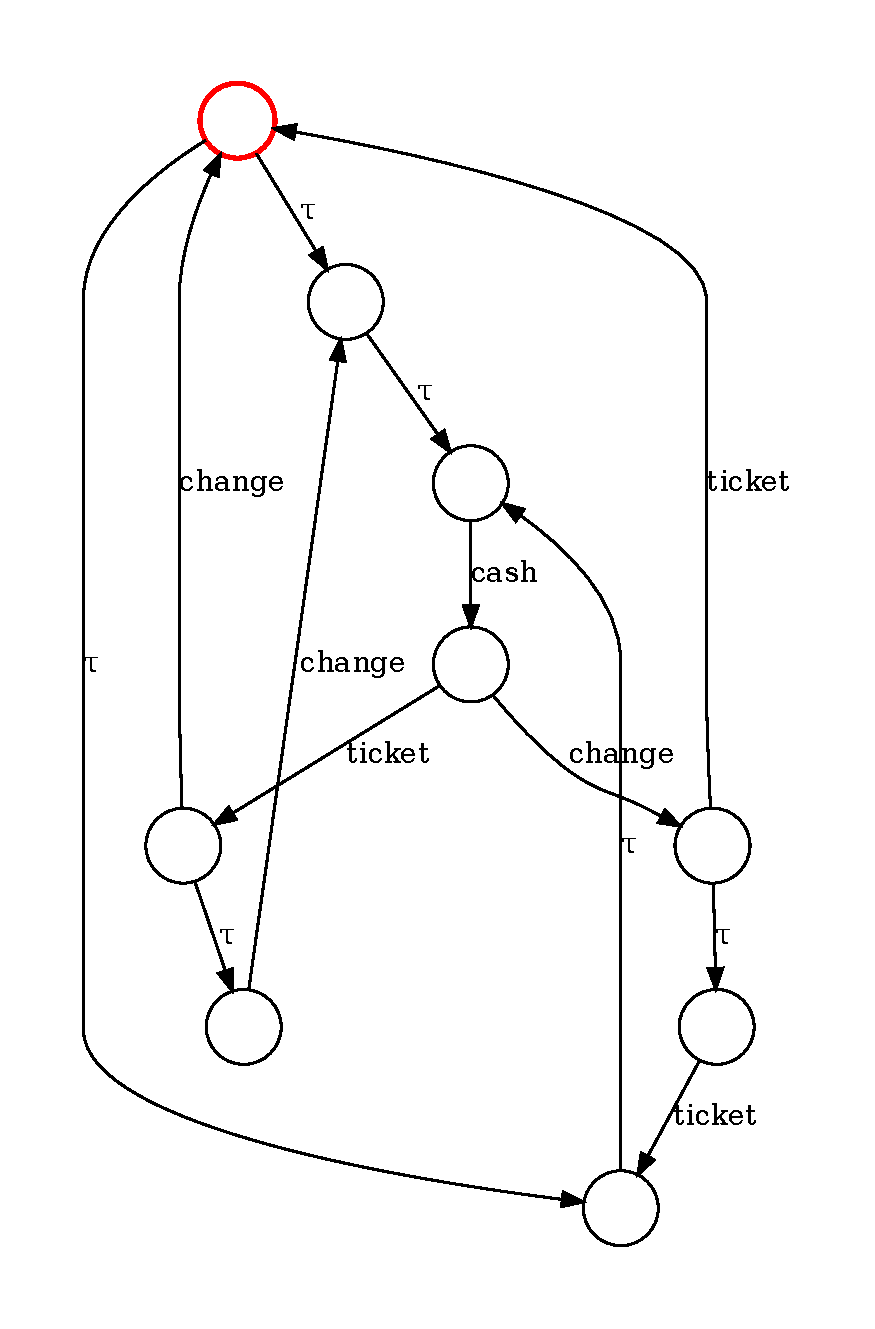
\includegraphics[scale=0.55]{images/parking_permit_mch_lts.pdf}
	\end{center}
\end{figure}

In \CSPcoq, it is also possible to generate such a graph displaying the behaviours (process bodies) associated with each state. Although this decreases the graph readability, it permits the user to know precisely the behaviour represented by each state.

% ---
\section{Traces refinement}
\label{section:traces}
% ---

As we have seen in Section~\ref{subsection:traces-refinement}, a simple but effective way to analyse the behaviour of a process is through the sequence of externally visible events that such a process is capable of performing over time. This communication history is called \emph{trace}. We may perceive a trace as a list of actions that takes from one state to another in an LTS. In Section~\ref{section:traces-concepts} we present our characterisation of traces in Coq, and in Section~\ref{section:quickchick} we explain how we use QuickChick to analyse traces-refinement expressions.

% ---
\subsection{Traces-related concepts}
\label{section:traces-concepts}
% ---

Like the other concepts of CSP we have discussed so far, traces are also formalised in \CSPcoq{}. This concept is defined in terms of a list of events that can be observed by the environment and, thus, $ \tau $ is not considered here. Although our definition of \emph{trace} allows the presence of $\tau$, the way we build traces prevents its appearance.

\begin{coqdoccode}
	\coqdocnoindent
	\coqdockw{Definition} \coqdocvar{trace} := \coqdocvar{list} \coqdocvar{event\_tau\_tick}.\coqdoceol
\end{coqdoccode}

After defining this new type, we can formalise being a trace as a relationship between a process P and a list of events L, so that it is possible to create logical propositions that involve assessing whether L is a trace of P. This relationship encodes the following inference rules:

\begin{itemize}
	\item the empty list is a trace of any process;
	\begin{prooftree}
		\AxiomC{}
		\UnaryInfC{$ \mathit{trace} \ P \ nil $}
	\end{prooftree}

	\item a non-empty list $L = h :: tl$ is a trace of a process $P$ if $P$ behaves as $Q$ after communicating $h$, which cannot be $\tau$, and the remaining events of this list is a trace of the process resulting from this communication;
	\begin{prooftree}
		\AxiomC{$ P \trans[h] Q $}
		\AxiomC{$ \mathit{trace} \ Q \ tl $}
		\RightLabel{\quad ($ h \notin \{\tau\} $)}
		\BinaryInfC{$ \mathit{trace} \ P \ (h :: tl) $}
	\end{prooftree}

	\item similarly, a list $L$ is a trace of a process $P$ if $ \tau $ can be performed by $P$ and $L$ is a trace of the process resulting from this communication.
	\begin{prooftree}
		\AxiomC{$ P \trans[\tau] Q $}
		\AxiomC{$ \mathit{trace} \ Q \ L $}
		\BinaryInfC{$ \mathit{trace} \ P \ L $}
	\end{prooftree}
\end{itemize}

To illustrate this concept, consider once again the process MACHINE, whose LTS is represented by the graph in Figure~\ref{image:machine_lts}. Examining this figure, one can note that the sequence of events <cash, ticket, change> is a trace of this process. First, the process communicates the internal event $ \tau $ twice, in order to unfold both sides of the parallel combination. Then, it proceeds to communicate the event cash, as the joint step of the MACHINE components (processes TICKET and CHANGE). Finally, the left-hand side of the parallel composition may communicate first, performing the event ticket; followed by event change, communicated by the right-hand side of the parallel composition. Remember that a trace consists of visible events only (also considering $\tick$), therefore the first two communicated events, which both happen to be $ \tau $, do not appear in the trace.

Now, we create an inductively defined proposition to formalise the traces notion, encoding the aforementioned rules, which are translated to three constructors of \coqdocvar{traceR'}. The propositional function \coqdocvar{traceR} is responsible for retrieving the process body associated with the provided process name.

\begin{coqdoccode}
	\coqdocnoindent
	\coqdockw{Inductive} \coqdocvar{traceR'} : \coqdocvar{specification} \ensuremath{\rightarrow} \coqdocvar{proc\_body} \ensuremath{\rightarrow} \coqdocvar{trace} \ensuremath{\rightarrow} \coqdockw{Prop} :=\coqdoceol
	\coqdocindent{1.00em}
	\ensuremath{|} \coqdocvar{empty\_trace\_rule} (\coqdocvar{S} : \coqdocvar{specification}) (\coqdocvar{P} : \coqdocvar{proc\_body}) :\coqdoceol
	\coqdocindent{2.00em}
	\coqdocvar{traceR'} \coqdocvar{S} \coqdocvar{P} \coqdocvar{nil}\coqdoceol
	\coqdocindent{1.00em}
	\ensuremath{|} \coqdocvar{event\_trace\_rule} (\coqdocvar{S} : \coqdocvar{specification}) (\coqdocvar{P} \coqdocvar{P'} : \coqdocvar{proc\_body}) (\coqdocvar{h} : \coqdocvar{event\_tau\_tick}) (\coqdocvar{tl} : \coqdocvar{trace}) :\coqdoceol
	\coqdocindent{2.00em}
	\ensuremath{\lnot} \coqdocvar{eq} \coqdocvar{h} \coqdocvar{Tau} \ensuremath{\rightarrow}\coqdoceol
	\coqdocindent{2.00em}
	(\coqdocvar{S} \# \coqdocvar{P} // \coqdocvar{h} ==> \coqdocvar{P'}) \ensuremath{\rightarrow}\coqdoceol
	\coqdocindent{2.00em}
	\coqdocvar{traceR'} \coqdocvar{S} \coqdocvar{P'} \coqdocvar{tl} \ensuremath{\rightarrow}\coqdoceol
	\coqdocindent{2.00em}
	\coqdocvar{traceR'} \coqdocvar{S} \coqdocvar{P} (\coqdocvar{h}::\coqdocvar{tl})\coqdoceol
	\coqdocindent{1.00em}
	\ensuremath{|} \coqdocvar{tau\_trace\_rule} (\coqdocvar{S} : \coqdocvar{specification}) (\coqdocvar{P} \coqdocvar{P'} : \coqdocvar{proc\_body}) (\coqdocvar{t} : \coqdocvar{trace}) :\coqdoceol
	\coqdocindent{2.00em}
	(\coqdocvar{S} \# \coqdocvar{P} // \coqdocvar{Tau} ==> \coqdocvar{P'}) \ensuremath{\rightarrow}\coqdoceol
	\coqdocindent{2.00em}
	\coqdocvar{traceR'} \coqdocvar{S} \coqdocvar{P'} \coqdocvar{t} \ensuremath{\rightarrow}\coqdoceol
	\coqdocindent{2.00em}
	\coqdocvar{traceR'} \coqdocvar{S} \coqdocvar{P} \coqdocvar{t}.\coqdoceol
	\coqdocemptyline
	\coqdocnoindent
	\coqdockw{Definition} \coqdocvar{traceR} (\coqdocvar{S} : \coqdocvar{specification}) (\coqdocvar{proc\_name} : \coqdocvar{string}) (\coqdocvar{t} : \coqdocvar{trace}) :=\coqdoceol
	\coqdocindent{1.00em}
	\coqdockw{match} (\coqdocvar{get\_proc\_body} \coqdocvar{S} \coqdocvar{proc\_name}) \coqdockw{with}\coqdoceol
	\coqdocindent{1.00em}
	\ensuremath{|} \coqdocvar{Some} \coqdocvar{body} \ensuremath{\Rightarrow} \coqdocvar{traceR'} \coqdocvar{S} \coqdocvar{body} \coqdocvar{t}\coqdoceol
	\coqdocindent{1.00em}
	\ensuremath{|} \coqdocvar{None} \ensuremath{\Rightarrow} \coqdocvar{False}\coqdoceol
	\coqdocindent{1.00em}
	\coqdockw{end}.\coqdoceol
\end{coqdoccode}

Note that the inference rules described before, in the order they were presented, correspond, respectively, to the constructors \coqdocvar{empty\_trace\_rule,} \coqdocvar{event\_trace\_rule}, and \coqdocvar{tau\_trace\_rule} of the \coqdocvar{traceR'} inductive definition.

This definition of traces as a relation allows us not only to make assertions like \emph{traceR S ``P'' L}, given a specification $ S $, a process $ P $ and a list of events $ L $, but also prove them in Coq by applying the constructors from the inductive declarations of traces and SOS.

It turns out that, the proof that $L$ is a trace of $P$ grows proportionally to the size of the list (trace). Additionally, these proofs also become quite repetitive. Fortunately, this repetition allows us to define an algorithm (decision procedure) to automatically prove assertions of this kind. Therefore, we have created a tactic macro for this purpose.

This algorithm can be defined as follows. If the goal is to prove the trace relation for an empty list, apply the rule \coqdocvar{empty\_trace\_rule} and finish the proof. Otherwise, try to make progress by applying each of the other two constructors of \coqdocvar{traceR'}, and then repeating this procedure until the proof is finished. For goals that involve expressions in terms of the \CSPcoq{} semantics (SOS), based o pattern matching, try to make progress using the SOS constructors applicable for the current SOS operator, making once again a recursive call at the end of this step.

The definition \coqdocvar{solve\_trace'}, partially presented in what follows, uses the Ltac language to describe this algorithm as a tactic macro that automatically proves statements of the kind \emph{traceR S ``P'' L}. Note that the first case deals with the situation when the list is empty (\emph{nil}). The second case tries to make progress by applying the \coqdocvar{tau\_trace\_rule} and \coqdocvar{event\_trace\_rule} constructors. Then, we have many cases considering the application of SOS constructors. In the end, we have some additional cases for proving some specific propositions, involving \coqdocvar{set\_In} and disjunctions. Finally, the tactic \coqdocvar{solve\_trace} works unfolding the definition \emph{traceR}, performing simplification and, then, invoking the tactic \coqdocvar{solve\_trace'}.

\begin{coqdoccode}
	\coqdocnoindent
	\coqdockw{Ltac} \coqdocvar{solve\_trace'} :=\coqdoceol
	\coqdocindent{1.00em}
	\coqdocvar{multimatch} \coqdockw{goal} \coqdockw{with}\coqdoceol
	\coqdocindent{1.00em}
	\ensuremath{|} \ensuremath{\vdash} \coqdocvar{traceR'} \coqdocvar{\_} \coqdocvar{\_} \coqdocvar{nil} \ensuremath{\Rightarrow} \coqdoctac{apply} \coqdocvar{empty\_trace\_rule}\coqdoceol
	\coqdocindent{1.00em}
	\ensuremath{|} \ensuremath{\vdash} \coqdocvar{traceR'} \coqdocvar{\_} \coqdocvar{\_} \coqdocvar{\_} \ensuremath{\Rightarrow}\coqdoceol
	\coqdocindent{2.00em}
	(\coqdoctac{eapply} \coqdocvar{tau\_trace\_rule}\coqdoceol
	\coqdocindent{2.00em}
	+ \coqdoctac{eapply} \coqdocvar{event\_trace\_rule}); \coqdocvar{solve\_trace'}\coqdoceol
	\coqdocindent{1.00em}
	\ensuremath{|} \ensuremath{\vdash} \coqdocvar{\_} \# \coqdocvar{\_} --> \coqdocvar{\_} // \coqdocvar{\_} ==> \coqdocvar{\_} \ensuremath{\Rightarrow} \coqdoctac{apply} \coqdocvar{prefix\_rule}\coqdoceol
	\coqdocindent{1.00em}
	\ensuremath{|} \ensuremath{\vdash} \coqdocvar{\_} \# \coqdocvar{ProcRef} \coqdocvar{\_} // \coqdocvar{\_} ==> \coqdocvar{\_} \ensuremath{\Rightarrow} \coqdoctac{eapply} \coqdocvar{reference\_rule}; \coqdocvar{solve\_trace'}\coqdoceol
	\coqdocindent{1.00em}
	\ensuremath{|} \ensuremath{\vdash} \coqdocvar{\_} \# \coqdocvar{\_} [] \coqdocvar{\_} // \coqdocvar{\_} ==> \coqdocvar{\_} \ensuremath{\Rightarrow}\coqdoceol
	\coqdocindent{2.00em}
	(\coqdoctac{eapply} \coqdocvar{ext\_choice\_tau\_left\_rule}\coqdoceol
	\coqdocindent{2.00em}
	+ \coqdoctac{eapply} \coqdocvar{ext\_choice\_tau\_right\_rule}\coqdoceol
	\coqdocindent{2.00em}
	+ \coqdoctac{eapply} \coqdocvar{ext\_choice\_left\_rule}\coqdoceol
	\coqdocindent{2.00em}
	+ \coqdoctac{eapply} \coqdocvar{ext\_choice\_right\_rule}); \coqdocvar{solve\_trace'}\coqdoceol
	\coqdocindent{1.00em}
	$\vdots$\coqdoceol
	\coqdocindent{1.00em}
	\ensuremath{|} \ensuremath{\vdash} \coqdocvar{\_} \ensuremath{\not=} \coqdocvar{\_} \ensuremath{\Rightarrow} \coqdoctac{unfold} \coqdocvar{not}; \coqdockw{let} \coqdocvar{H} := \coqdoctac{fresh} ``H'' \coqdoctac{in} (\coqdoctac{intros} \coqdocvar{H}; \coqdoctac{inversion} \coqdocvar{H})\coqdoceol
	\coqdocindent{1.00em}
	\ensuremath{|} \ensuremath{\vdash} \coqdocvar{\_} = \coqdocvar{\_} \ensuremath{\Rightarrow} \coqdoctac{reflexivity}\coqdoceol
	\coqdocindent{1.00em}
	\ensuremath{|} \ensuremath{\vdash} \coqdocvar{set\_In} \coqdocvar{\_} \coqdocvar{\_} \ensuremath{\Rightarrow} \coqdoctac{simpl}; \coqdocvar{solve\_trace'}\coqdoceol
	\coqdocindent{1.00em}
	\ensuremath{|} \ensuremath{\vdash} \ensuremath{\lnot} \coqdocvar{set\_In} \coqdocvar{\_} \coqdocvar{\_} \ensuremath{\Rightarrow} \coqdocvar{solve\_not\_in}\coqdoceol
	\coqdocindent{1.00em}
	\ensuremath{|} \ensuremath{\vdash} \coqdocvar{\_} \ensuremath{\lor} \coqdocvar{\_} \ensuremath{\Rightarrow} (\coqdoctac{left} + \coqdoctac{right}); \coqdocvar{solve\_trace'}\coqdoceol
	\coqdocindent{1.00em}
	\coqdockw{end}.\coqdoceol
	\coqdocemptyline
	\coqdocnoindent
	\coqdockw{Ltac} \coqdocvar{solve\_trace} := \coqdoctac{unfold} \coqdocvar{traceR}; \coqdoctac{simpl}; \coqdocvar{solve\_trace'}.\coqdoceol
\end{coqdoccode}

The following proof revisits the trace example we have discussed earlier in this section. Using our tactic macro \coqdocvar{solve\_trace}, we can automatically prove that the list of events <cash, ticket, change> is indeed a trace of the process MACHINE (\autoref{image:machine_lts}).

\begin{coqdoccode}
	\coqdocnoindent
	\coqdockw{Example} \coqdocvar{MACHINE\_TRACE} :\coqdoceol
	\coqdocindent{1.00em}
	\coqdocvar{traceR} \coqdocvar{PARKING\_PERMIT\_MCH} ``MACHINE'' [``cash'' ; ``ticket'' ; ``change''].\coqdoceol
	\coqdocnoindent
	\coqdockw{Proof}. \coqdocvar{solve\_trace}. \coqdockw{Qed}.\coqdoceol
\end{coqdoccode}

Provided the definitions we have presented so far, we can finally formulate in Coq the concept of refinement according to the traces model, along with an appropriate notation for this relationship.

\begin{coqdoccode}
	\coqdocnoindent
	\coqdockw{Definition} \coqdocvar{trace\_refinement} (\coqdocvar{S} : \coqdocvar{specification}) (\coqdocvar{Spec} \coqdocvar{Imp} : \coqdocvar{string}) : \coqdockw{Prop} :=\coqdoceol
	\coqdocindent{1.00em}
	\coqdockw{\ensuremath{\forall}} (\coqdocvar{t} : \coqdocvar{trace}), \coqdocvar{traceR} \coqdocvar{S} \coqdocvar{Imp} \coqdocvar{t} \ensuremath{\rightarrow} \coqdocvar{traceR} \coqdocvar{S} \coqdocvar{Spec} \coqdocvar{t}.\coqdoceol
	\coqdocemptyline
	\coqdocnoindent
	\coqdockw{Notation} ``S `\#' P `[T=' Q'' := (\coqdocvar{trace\_refinement} \coqdocvar{S} \coqdocvar{P} \coqdocvar{Q})\coqdoceol
	\coqdocindent{1.00em}
	(\coqdoctac{at} \coqdockw{level} 150, \coqdoctac{left} \coqdockw{associativity}).\coqdoceol
\end{coqdoccode}

As we have explained in Section~\ref{subsection:traces-refinement}, this definition states that an implementation Q refines a specification P, according to the traces model, if, and only if, every trace of Q is also a trace of P.

% ---
\subsection{Checking refinement with QuickChick}
\label{section:quickchick}
% ---

In the context of this work, the QuickChick library was used to random test the refinement property according to the traces model. Our goal is to obtain a simple and automated way to test this property that relates two processes, Imp and Spec, eventually finding counterexamples for the traces refinement relation. In other words, we have developed a checker in QuickChick that tries to find a counterexample of a refinement expression by means of random property-based testing.

In order to create this checker, we first need to define a generator of random inputs, which, in our case, consist of traces for a given process. Thus, we define a random generator that takes a ``specification'' process and an arbitrary natural number to limit the maximum number of events in the trace. This generator returns a trace for the given process, whose size is limited by the third parameter. Proving that this generator is correct (i.e., all traces generated for a process $P$ are indeed traces of $P$ according to definition \coqdocvar{traceR}) remains as a future work.

The function \coqdocvar{gen\_valid\_trace} defines our generator by yielding an instance of the G Monad\footnote{More information available at \url{https://softwarefoundations.cis.upenn.edu/qc-current/QC.html}}. This function, as others presented before, retrieves the process body associated with the provided process identifier. Then, it calls the auxiliary function \coqdocvar{gen\_valid\_trace'}.

\begin{coqdoccode}
	\coqdocnoindent
	\coqdockw{Definition} \coqdocvar{gen\_valid\_trace}\coqdoceol
	\coqdocindent{1.00em}
	(\coqdocvar{S} : \coqdocvar{specification}) (\coqdocvar{proc\_id} : \coqdocvar{string}) (\coqdocvar{size} : \coqdocvar{nat})\coqdoceol
	\coqdocindent{1.00em}
	: \coqdocvar{G} (\coqdocvar{option} \coqdocvar{semantics\_trace.trace}) :=\coqdoceol
	\coqdocindent{1.00em}
	\coqdockw{match} \coqdocvar{get\_proc\_body} \coqdocvar{S} \coqdocvar{proc\_id} \coqdockw{with}\coqdoceol
	\coqdocindent{1.00em}
	\ensuremath{|} \coqdocvar{None} \ensuremath{\Rightarrow} \coqdocvar{ret} \coqdocvar{None}\coqdoceol
	\coqdocindent{1.00em}
	\ensuremath{|} \coqdocvar{Some} \coqdocvar{P} \ensuremath{\Rightarrow} \coqdocvar{gen\_valid\_trace'} \coqdocvar{S} \coqdocvar{P} \coqdocvar{size}\coqdoceol
	\coqdocindent{1.00em}
	\coqdockw{end}.\coqdoceol
\end{coqdoccode}

The function \coqdocvar{gen\_valid\_trace'} operates as follows. While the third parameter is greater than zero, decide -- based on a given frequency -- whether the generation should stop. If it should continue, generate a transition from the current state of the process, decreasing the argument that limits the trace size; call the generator recursively, passing the state reached by the transition generated in the previous step. Finally, return the concatenation of the event from this transition with the result of the recursive call, if the event is not $\tau$. The function \coqdocvar{freq\_} is responsible for making the probabilistic choice. In our case, the option to end the generation before reaching the limit has $ ((1 / (size + 1)) * 100)\% $ chance to happen, while continuing with the generation has the probability of $ ((size / (size + 1)) * 100)\% $.

\begin{coqdoccode}
	\coqdocnoindent
	\coqdockw{Fixpoint} \coqdocvar{gen\_valid\_trace'}\coqdoceol
	\coqdocindent{1.00em}
	(\coqdocvar{S} : \coqdocvar{specification}) (\coqdocvar{P} : \coqdocvar{proc\_body}) (\coqdocvar{size} : \coqdocvar{nat})\coqdoceol
	\coqdocindent{1.00em}
	: \coqdocvar{G} (\coqdocvar{option} \coqdocvar{semantics\_trace.trace}) :=\coqdoceol
	\coqdocindent{1.00em}
	\coqdockw{match} \coqdocvar{size} \coqdockw{with}\coqdoceol
	\coqdocindent{1.00em}
	\ensuremath{|} \coqdocvar{O} \ensuremath{\Rightarrow} \coqdocvar{ret} \coqdocvar{nil}\coqdoceol
	\coqdocindent{1.00em}
	\ensuremath{|} \coqdocvar{S} \coqdocvar{size'} \ensuremath{\Rightarrow}\coqdoceol
	\coqdocindent{2.00em}
	\coqdocvar{freq\_} (\coqdocvar{ret} \coqdocvar{nil}) [\coqdoceol
	\coqdocindent{3.00em}
	(1, \coqdocvar{ret} \coqdocvar{nil}) ;\coqdoceol
	\coqdocindent{3.00em}
	(\coqdocvar{size},\coqdoceol
	\coqdocindent{4.00em}
	\coqdocvar{bind} (\coqdocvar{gen\_valid\_trans} \coqdocvar{S} \coqdocvar{P}) (\coqdoceol
	\coqdocindent{5.00em}
	\coqdockw{fun} \coqdocvar{t} \ensuremath{\Rightarrow} (\coqdoceol
	\coqdocindent{6.00em}
	\coqdockw{match} \coqdocvar{t} \coqdockw{with}\coqdoceol
	\coqdocindent{6.00em}
	\ensuremath{|} \coqdocvar{nil} \ensuremath{\Rightarrow} \coqdocvar{ret} \coqdocvar{nil}\coqdoceol
	\coqdocindent{6.00em}
	\ensuremath{|} (\coqdocvar{Event} \coqdocvar{e}, \coqdocvar{Q}) :: \coqdocvar{\_} \ensuremath{\Rightarrow}\coqdoceol
	\coqdocindent{7.00em}
	\coqdocvar{bind} (\coqdocvar{gen\_valid\_trace'} \coqdocvar{S} \coqdocvar{Q} \coqdocvar{size'}) (\coqdoceol
	\coqdocindent{8.00em}
	\coqdockw{fun} \coqdocvar{ts} \ensuremath{\Rightarrow} \coqdocvar{ret} (\coqdocvar{Event} \coqdocvar{e} :: \coqdocvar{ts})\coqdoceol
	\coqdocindent{7.00em}
	)\coqdoceol
	\coqdocindent{6.00em}
	\ensuremath{|} (\coqdocvar{Tick}, \coqdocvar{Q}) :: \coqdocvar{\_} \ensuremath{\Rightarrow}\coqdoceol
	\coqdocindent{7.00em}
	\coqdocvar{bind} (\coqdocvar{gen\_valid\_trace'} \coqdocvar{S} \coqdocvar{Q} \coqdocvar{size'}) (\coqdoceol
	\coqdocindent{8.00em}
	\coqdockw{fun} \coqdocvar{ts} \ensuremath{\Rightarrow} \coqdocvar{ret} (\coqdocvar{Tick} :: \coqdocvar{ts})\coqdoceol
	\coqdocindent{7.00em}
	)\coqdoceol
	\coqdocindent{6.00em}
	\ensuremath{|} (\coqdocvar{Tau}, \coqdocvar{Q}) :: \coqdocvar{\_} \ensuremath{\Rightarrow}\coqdoceol
	\coqdocindent{7.00em}
	\coqdocvar{bind} (\coqdocvar{gen\_valid\_trace'} \coqdocvar{S} \coqdocvar{Q} \coqdocvar{size'}) (\coqdoceol
	\coqdocindent{8.00em}
	\coqdockw{fun} \coqdocvar{ts} \ensuremath{\Rightarrow} \coqdocvar{ret} \coqdocvar{ts}\coqdoceol
	\coqdocindent{7.00em}
	)\coqdoceol
	\coqdocindent{6.00em}
	\coqdockw{end}\coqdoceol
	\coqdocindent{5.00em}
	)\coqdoceol
	\coqdocindent{4.00em}
	)\coqdoceol
	\coqdocindent{3.00em}
	)\coqdoceol
	\coqdocindent{2.00em}
	]\coqdoceol
	\coqdocindent{1.00em}
	\coqdockw{end}.\coqdoceol
\end{coqdoccode}

The command that samples traces according to this generator, as well as part of the output of this sampling process are exemplified below.

\begin{coqdoccode}
	\coqdocnoindent
	\coqdocvar{Sample} (\coqdocvar{gen\_valid\_trace} \coqdocvar{PARKING\_PERMIT\_MCH} ``MACHINE'' 10).\coqdoceol
\end{coqdoccode}

\begin{tabbing}
	\emph{Output:}\\
	\emph{[Some []; Some [``cash''; ``change''; ``ticket''; ``cash''; ``change''];}\\
	\emph{Some [``cash'']; Some [``cash''; ``ticket''; ``change''; ``cash'']; Some [];}\\
	\emph{Some [``cash''; ``change''; ``ticket''; ``cash'']; Some [``cash''; ``change''; ``ticket'']; $\dots$]}
\end{tabbing}

As one can see, the definition of \coqdocvar{gen\_valid\_trace'} relies on a generator of random transitions from a given process $P$ (\coqdocvar{gen\_valid\_trans}). The latter generator receives a specification and a process body, and yields a list containing exactly one valid random transition from the given state, where the transition is represented by the pair (action, target\_state). The generation of all emanating transitions from a given process $P$ is performed by \coqdocvar{get\_transitions}, which is a function used in our computable definition of LTSs.

\begin{coqdoccode}
	\coqdocnoindent
	\coqdockw{Definition} \coqdocvar{gen\_valid\_trans}\coqdoceol
	\coqdocindent{1.00em}
	(\coqdocvar{S} : \coqdocvar{specification})\coqdoceol
	\coqdocindent{1.00em}
	(\coqdocvar{P} : \coqdocvar{proc\_body})\coqdoceol
	\coqdocindent{1.00em}
	: \coqdocvar{G} (\coqdocvar{option} (\coqdocvar{list} (\coqdocvar{event\_tau\_tick} \ensuremath{\times} \coqdocvar{proc\_body}))) :=\coqdoceol
	\coqdocindent{1.00em}
	\coqdockw{match} \coqdocvar{get\_transitions} \coqdocvar{S} \coqdocvar{P} \coqdockw{with}\coqdoceol
	\coqdocindent{1.00em}
	\ensuremath{|} \coqdocvar{None} \ensuremath{\Rightarrow} \coqdocvar{ret} \coqdocvar{None}\coqdoceol
	\coqdocindent{1.00em}
	\ensuremath{|} \coqdocvar{Some} \coqdocvar{nil} \ensuremath{\Rightarrow} \coqdocvar{ret} \coqdocvar{nil}\coqdoceol
	\coqdocindent{1.00em}
	\ensuremath{|} \coqdocvar{Some} (\coqdocvar{t} :: \coqdocvar{ts}) \ensuremath{\Rightarrow} \coqdocvar{bind} (\coqdocvar{elems\_} \coqdocvar{t} (\coqdocvar{t} :: \coqdocvar{ts})) (\coqdockw{fun} \coqdocvar{a} \ensuremath{\Rightarrow} \coqdocvar{ret} (\coqdocvar{Some} [\coqdocvar{a}]))\coqdoceol
	\coqdocindent{1.00em}
	\coqdockw{end}.\coqdoceol
\end{coqdoccode}

\noindent The following lines exemplify the usage of \coqdocvar{gen\_valid\_trans}.

\begin{coqdoccode}
	\coqdocnoindent
	\coqdocvar{Sample} (\coqdocvar{gen\_valid\_trans} \coqdocvar{PARKING\_PERMIT\_MCH}\coqdoceol
	\coqdocindent{1.00em}
	(\coqdocvar{ProcRef} ``TICKET''\coqdoceol
	\coqdocindent{1.40em} [[ \{\{``cash'', ``ticket''\}\} \symbol{92}\symbol{92} \{\{``cash'', ``change''\}\} ]]\coqdoceol
	\coqdocindent{1.40em}\coqdocvar{ProcRef} ``CHANGE'')).\coqdoceol
\end{coqdoccode}

\begin{tabbing}
	\emph{Output:}\\
	\emph{[Some [($ \tau $,TICKET [{ticket, cash} || {change, cash}] cash $ \rightarrow $ change $ \rightarrow $ CHANGE)];}\\
	\emph{Some [($ \tau $,cash $ \rightarrow $ ticket $ \rightarrow $ TICKET [{ticket, cash} || {change, cash}] CHANGE)]; $\dots$]}
\end{tabbing}

Note that, since this generator also computes transitions in which $ \tau $ may appear as actions, it is necessary to hide them, so that the generated trace does not consider these internal events. The generator \coqdocvar{gen\_valid\_trace} does so by concatenating only external events and $\tick$ to the list that will be returned.

Once the random generator of traces is defined, we need an executable property that uses the generated traces to assess a refinement expression. Therefore, we define the function \coqdocvar{check\_trace'} to check whether the trace generated from a process \emph{Imp} is also a trace of a process \emph{Spec}. The idea behind this function is to try to make progress within the given process, one step at a time, consuming the events of the trace in the order in which they appear, while trying to guess non-deterministically when it is necessary to insert a $ \tau $ for the sequence of events to be accepted by the process.

The function \coqdocvar{check\_trace'} initially computes all possible immediate transitions from one state. Then, it filters, from these transitions, those whose action corresponds either to the current element in the list of events (trace), or the internal event. Then, we try to make progress with each of these valid events, performing a recursive call considering each target state obtained from the transitions in the previous step, but removing the corresponding event from the list when applicable -- that is, except $ \tau $. If any of the recursive calls reach an empty list (trace), then the provided trace is indeed a trace of the process. Differently, if none of the recursive calls is able to make progress, then we can assume that this list is not a trace of the process.

\begin{coqdoccode}
	\coqdocnoindent
	\coqdockw{Fixpoint} \coqdocvar{check\_trace'}\coqdoceol
	\coqdocindent{1.00em}
	(\coqdocvar{S} : \coqdocvar{specification})	(\coqdocvar{P} : \coqdocvar{proc\_body})	(\coqdocvar{event\_list} : \coqdocvar{trace}) (\coqdocvar{fuel} : \coqdocvar{nat}) : \coqdocvar{option} \coqdocvar{bool} :=\coqdoceol
	\coqdocindent{1.00em}
	\coqdockw{match} \coqdocvar{fuel}, \coqdocvar{event\_list} \coqdockw{with}\coqdoceol
	\coqdocindent{1.00em}
	\ensuremath{|} \coqdocvar{\_}, \coqdocvar{nil} \ensuremath{\Rightarrow} \coqdocvar{Some} \coqdocvar{true}\coqdoceol
	\coqdocindent{1.00em}
	\ensuremath{|} \coqdocvar{O}, \coqdocvar{\_} \ensuremath{\Rightarrow} \coqdocvar{None} \coqdoceol
	\coqdocindent{1.00em}
	\ensuremath{|} \coqdocvar{S} \coqdocvar{fuel'}, \coqdocvar{e} :: \coqdocvar{es} \ensuremath{\Rightarrow}\coqdoceol
	\coqdocindent{2.00em}
	\coqdockw{match} \coqdocvar{get\_transitions} \coqdocvar{S} \coqdocvar{P} \coqdockw{with}\coqdoceol
	\coqdocindent{2.00em}
	\ensuremath{|} \coqdocvar{None} \ensuremath{\Rightarrow} \coqdocvar{None}\coqdoceol
	\coqdocindent{2.00em}
	\ensuremath{|} \coqdocvar{Some} \coqdocvar{t} \ensuremath{\Rightarrow}\coqdoceol
	\coqdocindent{3.00em}
	\coqdockw{let} \coqdocvar{available\_moves} := \coqdocvar{t} \coqdoctac{in}\coqdoceol
	\coqdocindent{3.00em}
	\coqdockw{let} \coqdocvar{valid\_moves} := \coqdocvar{filter} (\coqdoceol
	\coqdocindent{4.00em}
	\coqdockw{fun} \coqdocvar{t} \ensuremath{\Rightarrow} (\coqdocvar{is\_equal} (\coqdocvar{fst} \coqdocvar{t}) (\coqdocvar{Event} \coqdocvar{e}))\coqdoceol
	\coqdocindent{5.00em}
	|| (\coqdocvar{is\_equal} (\coqdocvar{fst} \coqdocvar{t}) \coqdocvar{Tau})\coqdoceol
	\coqdocindent{5.00em}
	|| (\coqdocvar{is\_equal} (\coqdocvar{fst} \coqdocvar{t}) \coqdocvar{Tick})\coqdoceol
	\coqdocindent{3.00em}
	) \coqdocvar{available\_moves} \coqdoctac{in}\coqdoceol
	\coqdocindent{3.00em}
	\coqdockw{match} \coqdocvar{valid\_moves} \coqdockw{with}\coqdoceol
	\coqdocindent{3.00em}
	\ensuremath{|} \coqdocvar{nil} \ensuremath{\Rightarrow} \coqdocvar{Some} \coqdocvar{false}\coqdoceol
	\coqdocindent{3.00em}
	\ensuremath{|} \coqdocvar{\_} \ensuremath{\Rightarrow}\coqdoceol
	\coqdocindent{4.00em}
	\coqdockw{let} \coqdocvar{result} := \coqdocvar{map} (\coqdockw{fun} \coqdocvar{t} \ensuremath{\Rightarrow}\coqdoceol
	\coqdocindent{5.00em}
	\coqdockw{if} \coqdocvar{negb} (\coqdocvar{is\_equal} (\coqdocvar{fst} \coqdocvar{t}) (\coqdocvar{Tau}))\coqdoceol
	\coqdocindent{5.00em}
	\coqdockw{then} \coqdocvar{check\_trace'} \coqdocvar{S} (\coqdocvar{snd} \coqdocvar{t}) \coqdocvar{es} \coqdocvar{fuel'}\coqdoceol
	\coqdocindent{5.00em}
	\coqdockw{else} \coqdocvar{check\_trace'} \coqdocvar{S} (\coqdocvar{snd} \coqdocvar{t}) (\coqdocvar{e} :: \coqdocvar{es}) \coqdocvar{fuel'}\coqdoceol
	\coqdocindent{4.00em}
	) \coqdocvar{valid\_moves} \coqdoctac{in}\coqdoceol
	\coqdocindent{4.00em}
	\coqdockw{if} \coqdocvar{existsb} (\coqdockw{fun} \coqdocvar{o} \ensuremath{\Rightarrow}\coqdoceol
	\coqdocindent{5.00em}
	\coqdockw{match} \coqdocvar{o} \coqdockw{with}\coqdoceol
	\coqdocindent{5.00em}
	\ensuremath{|} \coqdocvar{Some} \coqdocvar{true} \ensuremath{\Rightarrow} \coqdocvar{true}\coqdoceol
	\coqdocindent{5.00em}
	\ensuremath{|} \coqdocvar{\_} \ensuremath{\Rightarrow} \coqdocvar{false}\coqdoceol
	\coqdocindent{5.00em}
	\coqdockw{end}) \coqdocvar{result}\coqdoceol
	\coqdocindent{4.00em}
	\coqdockw{then} \coqdocvar{Some} \coqdocvar{true}\coqdoceol
	\coqdocindent{4.00em}
	\coqdockw{else} \coqdockw{if} \coqdocvar{forallb} (\coqdockw{fun} \coqdocvar{o} \ensuremath{\Rightarrow}\coqdoceol
	\coqdocindent{5.00em}
	\coqdockw{match} \coqdocvar{o} \coqdockw{with}\coqdoceol
	\coqdocindent{5.00em}
	\ensuremath{|} \coqdocvar{Some} \coqdocvar{false} \ensuremath{\Rightarrow} \coqdocvar{true}\coqdoceol
	\coqdocindent{5.00em}
	\ensuremath{|} \coqdocvar{\_} \ensuremath{\Rightarrow} \coqdocvar{false}\coqdoceol
	\coqdocindent{5.00em}
	\coqdockw{end}) \coqdocvar{result}\coqdoceol
	\coqdocindent{4.00em}
	\coqdockw{then} \coqdocvar{Some} \coqdocvar{false}\coqdoceol
	\coqdocindent{4.00em}
	\coqdockw{else} \coqdocvar{None}\coqdoceol
	\coqdocindent{3.00em}
	\coqdockw{end}\coqdoceol
	\coqdocindent{2.00em}
	\coqdockw{end}\coqdoceol
	\coqdocindent{1.00em}
	\coqdockw{end}.\coqdoceol
\end{coqdoccode}

The function \coqdocvar{check\_trace'} is called by \coqdocvar{check\_trace}, which retrieves the process body associated with the provided process identifier.

\begin{coqdoccode}
	\coqdocemptyline
	\coqdocnoindent
	\coqdockw{Definition} \coqdocvar{check\_trace}\coqdoceol
	\coqdocindent{1.00em}
	(\coqdocvar{S} : \coqdocvar{specification}) (\coqdocvar{proc\_id} : \coqdocvar{string}) (\coqdocvar{event\_list} : \coqdocvar{trace}) 	(\coqdocvar{fuel} : \coqdocvar{nat}) : \coqdocvar{option} \coqdocvar{bool} :=\coqdoceol
	\coqdocindent{1.00em}
	\coqdockw{match} \coqdocvar{fuel}, \coqdocvar{get\_proc\_body} \coqdocvar{S} \coqdocvar{proc\_id} \coqdockw{with}\coqdoceol
	\coqdocindent{1.00em}
	\ensuremath{|} \coqdocvar{O}, \coqdocvar{\_} \ensuremath{|} \coqdocvar{\_}, \coqdocvar{None} \ensuremath{\Rightarrow} \coqdocvar{None}\coqdoceol
	\coqdocindent{1.00em}
	\ensuremath{|} \coqdocvar{S} \coqdocvar{fuel'}, \coqdocvar{Some} \coqdocvar{P} \ensuremath{\Rightarrow} \coqdocvar{check\_trace'} \coqdocvar{S} \coqdocvar{P} \coqdocvar{event\_list} \coqdocvar{fuel'}\coqdoceol
	\coqdocindent{1.00em}
	\coqdockw{end}.\coqdoceol
\end{coqdoccode}

Finally, the function \coqdocvar{traceP} provides the given trace to \coqdocvar{check\_trace} and propagates the boolean yielded by the latter function.

\begin{coqdoccode}
	\coqdocnoindent
	\coqdockw{Definition} \coqdocvar{traceP}\coqdoceol
	\coqdocindent{1.00em}
	(\coqdocvar{S} : \coqdocvar{specification})
	(\coqdocvar{proc\_id} : \coqdocvar{string})
	(\coqdocvar{fuel} : \coqdocvar{nat})\coqdoceol
	\coqdocindent{1.00em}
	(\coqdocvar{t} : \coqdocvar{option} \coqdocvar{semantics\_trace.trace}) : \coqdocvar{bool} :=\coqdoceol
	\coqdocindent{1.00em}
	\coqdockw{match} \coqdocvar{t} \coqdockw{with}\coqdoceol
	\coqdocindent{1.00em}
	\ensuremath{|} \coqdocvar{None} \ensuremath{\Rightarrow} \coqdocvar{false}\coqdoceol
	\coqdocindent{1.00em}
	\ensuremath{|} \coqdocvar{Some} \coqdocvar{t'} \ensuremath{\Rightarrow}\coqdoceol
	\coqdocindent{2.00em}
	\coqdockw{match} \coqdocvar{check\_trace} \coqdocvar{S} \coqdocvar{proc\_id} \coqdocvar{t'} \coqdocvar{fuel} \coqdockw{with}\coqdoceol
	\coqdocindent{2.00em}
	\ensuremath{|} \coqdocvar{None} \ensuremath{\Rightarrow} \coqdocvar{false}\coqdoceol
	\coqdocindent{2.00em}
	\ensuremath{|} \coqdocvar{Some} \coqdocvar{b} \ensuremath{\Rightarrow} \coqdocvar{b}\coqdoceol
	\coqdocindent{2.00em}
	\coqdockw{end}\coqdoceol
	\coqdocindent{1.00em}
	\coqdockw{end}.\coqdoceol
\end{coqdoccode}

Provided these definitions, we define the refinement-property checker. This checker tests whether every randomly generated trace of an implementation process is also a trace of a specification process. This definition reflects the formal definition of the trace-refinement relation presented in Section~\ref{section:traces-concepts}.

\begin{coqdoccode}
	\coqdocnoindent
	\coqdockw{Definition} \coqdocvar{trace\_refinement\_checker}\coqdoceol
	\coqdocindent{1.00em}
	(\coqdocvar{S} : \coqdocvar{specification})
	(\coqdocvar{Imp} \coqdocvar{Spec} : \coqdocvar{string})
	(\coqdocvar{trace\_max\_size} : \coqdocvar{nat})
	(\coqdocvar{fuel} : \coqdocvar{nat}) : \coqdocvar{Checker} :=\coqdoceol
	\coqdocindent{2.00em}
	\coqdocvar{forAll} (\coqdocvar{gen\_valid\_trace} \coqdocvar{S} \coqdocvar{Imp} \coqdocvar{trace\_max\_size}) (\coqdocvar{traceP} \coqdocvar{S} \coqdocvar{Spec} \coqdocvar{fuel}).\coqdoceol
\end{coqdoccode}

To illustrate the verification of this executable property, consider the following \CSPcoq{} specification.

\begin{coqdoccode}
	\coqdocnoindent
	\coqdockw{Definition} \coqdocvar{EXAMPLE} : \coqdocvar{specification}.\coqdoceol
	\coqdocnoindent
	\coqdockw{Proof}.\coqdoceol
	\coqdocindent{1.00em}
	\coqdocvar{solve\_spec\_ctx\_rules} (\coqdoceol
	\coqdocindent{2.00em}
	\coqdocvar{Build\_Spec}\coqdoceol
	\coqdocindent{3.00em}
	[ \coqdocvar{Channel} \{\{``a'', ``b'', ``c''\}\} ]\coqdoceol
	\coqdocindent{3.00em}
	[ ``P'' ::= ``a'' -{}-> ``b'' -{}-> \coqdocvar{ProcRef} ``P'' ;\coqdoceol
	\coqdocindent{4.00em}
	``Q'' ::= (``a'' -{}-> ``b'' -{}-> \coqdocvar{ProcRef} ``Q'') [] (``c'' -{}-> \coqdocvar{STOP}) ]\coqdoceol
	\coqdocindent{1.00em}
	).\coqdoceol
	\coqdocnoindent
	\coqdockw{Defined}.\coqdoceol
\end{coqdoccode}

If we may want to check whether ``Q'' trace-refines ``P'', that is, if every trace of ``Q'' is also a trace of ``P'', we invoke our checker with the command \coqdocvar{QuickChick}, passing, for instance, 5 as the maximum trace size and the arbitrary integer 1000 as the fuel argument (to limit the number of performed recursions).

\begin{coqdoccode}
	\coqdocnoindent
	\coqdocvar{QuickChick} (\coqdocvar{trace\_refinement\_checker} \coqdocvar{EXAMPLE} ``Q'' ``P'' 5 1000).\coqdoceol
\end{coqdoccode}

\begin{tabbing}
	\emph{Some [``c'']} \\
	\emph{*** Failed after 3 tests and 0 shrinks. (0 discards)}
\end{tabbing}

As we are told by the message above, QuickChick performed 3 tests before running into a trace that violates the refinement relation, showing evidence that ``Q'' does not trace-refine ``P'', since [``c''] is a trace of ``Q'', but it is not a trace of ``P''. Differently, note that the process ``Q'' is actually refined by ``P'' (i.e. ``P'' trace-refines ``Q''). We will not be able to prove that statement with our checker though. Instead, it may only lead us to believe that the relation holds, since QuickChick is not able to provide us with any counterexample after executing 10000 tests.

\begin{coqdoccode}
	\coqdocnoindent
	\coqdocvar{QuickChick} (\coqdocvar{trace\_refinement\_checker} \coqdocvar{EXAMPLE} ``P'' ``Q'' 5 1000).\coqdoceol
\end{coqdoccode}

\begin{tabbing}
	\emph{+++ Passed 10000 tests (0 discards)}
\end{tabbing}

Therefore, since this method is, ultimately, a testing solution, we are only interested in counterexamples, which actually show evidence that the refinement relation does not hold between two processes. Passing tests must be considered nothing but a mere indication of a possibly valid refinement expression. In other words, this refinement-checking approach is sound (if the checked property does not hold, the trace-refinement relation does not hold), but it is not complete (if the checked property holds, we can not guarantee whether the trace-refinement relation holds).

Using Coq, allows us to develop proofs to show that a particular property, such that a process refines another one, holds. Nevertheless, using QuickChick, a testing-based tool, may be interesting as a first step towards the development of the proof. Before trying to prove a given statement, which may be trivially false, one can use such a tool to find basic counterexamples. If none is found, although this cannot be considered as a definitive proof, it gives us some empirical evidence that the statement may be true indeed. This idea may save time when trying to prove propositions that are false.

% ---
% Chapter 4
% ---
\chapter{Conclusions}
% ---

In this work, we embedded a subset of the CSP language in the Coq proof assistant, giving rise to the language entitled \CSPcoq{}. The abstract syntax was described through inductive types, while the concrete syntax relies on the concept of notations. In addition, the inductive declaration that defines operational semantics in the SOS style was also presented. The concept of LTS was represented both in an inductive and functional approach, supporting a third-party tool that allows a custom graphic visualization of this structure.

Finally, the notion of the trace of a process was declared, along with a tactic macro that automates the proof of this relation. These accomplishments led to the definition of the refinement relation according to the traces model, in addition to the implementation of two generators and one checker for this property, in order to test it using a property-based random testing plugin.

% ---
\section{Related work}
% ---

% Comentar a existência de trabalhos relacionados, mencionando CSP-Prover e Isabelle/UTP.
Several studies have shown how to embed the theories of many CSP models in theorem proving tools such as Isabelle \cite{Paulson:Isabelle}, and then prove both the laws of CSP in general and other coherency properties of the definitions of CSP operators over the models. In particular, we want to discuss two implementations that share the same motivation of this work: the CSP-Prover \cite{Roggenbach:CSP-Prover} and Isabelle/UTP verification toolbox \cite{Woodcock:Isabelle/UTP}.

% CSP-Prover
CSP-Prover is an interactive theorem prover dedicated to refinement proofs within CSP based on Isabelle. It focuses on the stable failures model $ \fmodel $ as the underlying denotational semantics of CSP, including the CSP traces model $ \tmodel $ as a by-product. Consequently, CSP-Prover contains the definitions of CSP syntax and semantics, and semi-automatic proof tactics for verification of refinement relation.

% Isabelle/UTP
Isabelle/UTP is an implementation of Hoare and He's \emph{Unifying Theories of Programming} framework based in Isabelle/HOL. UTP is a framework for construction of denotational semantic meta-models for a variety of programming languages based on an alphabetized relational calculus. This implementation can be used to formalize semantic building blocks for programming language paradigms, prove algebraic laws of programming, and then use these laws to construct program verification tools.

The \autoref{tab:framework_comparison} provides a comparison between the framework we developed, the CSP-Prover, and the Isabelle/UTP, highlighting the main features shared by these implementations:

\begin{table}[htb]
	\begin{center}
		\caption[A feature comparison between \CSPcoq{} and related work]{A feature comparison between \CSPcoq{} and related work.}
		\label{tab:framework_comparison}
		\begin{tabular}{ |l|c|c|c| }
			\hline
			Feature & \CSPcoq{} & CSP-Prover & Isabelle/UTP \\
			\hline
			CSP Dialect & Partial & Complete & Complete \\ [0.5ex]
			Operational semantics & Structured & Not Available & Relational \\ [0.5ex]
			Denotational semantics (model) & Traces & Stable failures/Traces & Not Available \\ [0.5ex]
			LTS representation & Available & Not available & Not Available \\ [0.5ex]
			Trace relation tactics & Available & Not Available & Not Available \\ [0.5ex]
			Refinement relation tactics & Not Available & Available & Available \\ [0.5ex]
			Random testing (refinement) & Available & Not Available & Not Available \\ [0.5ex]
			\hline
		\end{tabular}
	\end{center}
\end{table}

From the table above, we are able to conclude that the main advantages of \CSPcoq{} over others embedding of CSP theory in theorem proving tools mentioned here is its emphasis on the traces model as well as the LTS representation support, enabling the user to check a list of events for being a trace of a process, solving the trace relation proof automatically, and generating a graph of the LTS of a process.

% ---
\section{Future work}
% ---

%TODO -- proofs of correctness

The topics listed below describe relevant activities that extend the work we developed:
\begin{itemize}
	\item Extend the language \CSPcoq{} to include the remaining CSP operators. The theory of CSP, as well as the ASCII version of the language, contemplates more advanced concepts such as parameterized processes and operations like event renaming, interruption, exception, among others. It is necessary to include these concepts in order to leverage the framework developed.
	\item Prove that for every process $ P $, there is a list of transitions $ L $ such that if \emph{ltsR S P L}, then there is natural $ n $ such that \emph{compute\_ltsR S P n = Some L}. This proof guarantees the completeness of the definition \emph{compute\_ltsR}, and that is, every set of transitions that characterize the LTS of a process is computable from this definition.
	\item Define the tactic macro that automatically proves if the \emph{ltsR} relation holds for a given process. The proof for the ltsR relation can be long, and they usually follow a well-defined pattern. Creating a tactic macro would simplify tasks like checking if a set of transitions is indeed the LTS of a process.
	\item Formalize the concept of a extended trace, say \emph{extended\_traceR}, including the events $ \tau $ and $ \tick $; relate \emph{traceR} and \emph{extended\_traceR}; create tactic macro that automates the proofs for the new \emph{extended\_traceR} relation. A trace, by definition, does not include the events $ \tau $ and $ \tick $, which may sometimes simplify the actual behavior of a process. Therefore, an extended definition of trace would expose these suppressed communications.
	\item Implement verification of forbidden use of recursion in the context of hiding and parallelism operations. These operations, when appearing in a process recursion, introduce the issue of accumulated operators. For instance, the process definition $ P = (a \rightarrow P) \ \textbackslash \ \{a\} $, although syntactically correct, generates a new state in the LTS of the process $ P $ every time $ P $ is unfolded in the body, due to the addition of one more hiding operation to the process body: $ (a \rightarrow P) \ \textbackslash \ \{a\} \trans[a] ((a \rightarrow P) \ \textbackslash \ \{a\}) \ \textbackslash \ \{a\} \trans[a] (((a \rightarrow P) \ \textbackslash \ \{a\}) \ \textbackslash \ \{a\}) \ \textbackslash \ \{a\} \trans[a] \ \dots$
	\item Define traces refinement in terms of a bi-simulation. The notion of strong bi-simulation is, in order to be equivalent, two processes must have the same set of events available immediately, with these events leading to processes that are themselves equivalent. Since it is virtually impossible to implement a function that enumerates all traces of a process -- so that we could use it to make assertions about a refinement statement -- this equivalence over LTS would be the proper way to achieve this goal.
	\item Compress the generated LTS, removing intermediate $ \tau $'s. The process unwind and sequential composition operations introduce the communication of the internal event $ \tau $ as a way to take into account the ``effort'' of unfolding a process body inside another. Omitting these communications may, not only reduce the LTS size, but also make it more simple to spot equivalent process by looking at their LTS's.
	\item Prove that for all transition lists $ L1 $ and $ L2 $, if \emph{ltsR S P L1} and \emph{ltsR S P L2}, then $ L1 $ is a permutation of $ L2 $. Since our definition of LTS is based on a list of transitions instead of a set, this proof would guarantee that there aren't two lists of transitions with different elements that consists of the LTS of the same process. In other words, this would prove the uniqueness of the transition set of an LTS.
\end{itemize}

% ----------------------------------------------------------
% ELEMENTOS PÓS-TEXTUAIS
% ----------------------------------------------------------
\postextual
% ----------------------------------------------------------

% ----------------------------------------------------------
% Referências bibliográficas
% ----------------------------------------------------------
\bibliography{references}

\end{document}